\documentclass[11pt,a4paper]{article}

% Packages
\usepackage[utf8]{inputenc}
\usepackage[T1]{fontenc}
% \usepackage[french]{babel}  % Décommenter si babel fonctionne sur votre système
\usepackage{amsmath,amssymb}
\usepackage{bm}              % Pour \bm{} (bold math)
\usepackage{graphicx}
\usepackage{booktabs}
\usepackage{siunitx}
\usepackage{caption}
\usepackage{subcaption}
\usepackage{hyperref}
\usepackage[margin=2.5cm]{geometry}
\usepackage{float}
\usepackage{listings}
\usepackage[table]{xcolor}
\usepackage{comment}         % Pour \begin{comment}...\end{comment}
\usepackage{tcolorbox}       % Pour les boîtes colorées
\usepackage{mdframed}        % Pour les cadres
\usepackage{tikz}            % Pour les figures TikZ
\usetikzlibrary{arrows.meta, patterns, decorations.pathreplacing, calc, positioning, shapes.geometric}

% Définition des couleurs
\definecolor{brass}{RGB}{181, 166, 66}
\definecolor{tungsten}{RGB}{100, 100, 120}
\definecolor{beryllium}{RGB}{200, 220, 200}
\definecolor{aluminum}{RGB}{180, 180, 195}
\definecolor{water}{RGB}{100, 150, 220}
\definecolor{air}{RGB}{230, 240, 255}
\definecolor{steel}{RGB}{160, 160, 170}
\definecolor{darkblue}{RGB}{31,78,121}
\definecolor{darkred}{RGB}{192,0,0}
\definecolor{dose1}{RGB}{255, 107, 107}
\definecolor{dose2}{RGB}{255, 160, 122}
\definecolor{dose3}{RGB}{255, 215, 0}
\definecolor{dose4}{RGB}{144, 238, 144}
\definecolor{dose5}{RGB}{135, 206, 235}
\definecolor{header}{RGB}{70, 130, 180}
\definecolor{lightgray}{RGB}{245, 245, 245}
\definecolor{mediumblue}{RGB}{46,117,182}
\definecolor{lightblue}{RGB}{231,240,247}

% Configuration siunitx
\sisetup{
    locale = FR,
    separate-uncertainty = true,
    per-mode = symbol
}

\title{Analyse des distributions spatiales dans container d'eau\\
\large Simulation Monte Carlo de transport de particules}
\author{GM}
\date{\today}

\begin{document}

\maketitle


%\tableofcontents
\newpage



%==============================================================================
\normalsize
\noindent \begin{mdframed}[backgroundcolor=orange!20]
\section{\Large \color{blue} \textbf{Géométrie}\color{black}}
\end{mdframed}
\footnotesize

\begin{tcolorbox}[colback=blue!5,colframe=blue,title=\textbf{Configuration}]
\noindent ${\rm \; \; \; \; \; \; }$ \textbf{-} \; Analyse des \color{blue}\textbf{doses déposées}\color{black} \; dans un container d'eau à 68 mm apres la sortie du collimateur de 4mm le long de l'axe $\bm{z}$.\\
\noindent ${\rm \; \; \; \; \; \; }$ \textbf{-} \; le \color{blue}\textbf{diamètre de l'eau est de 20 mm}\color{black}\\ 
\noindent ${\rm \; \; \; \; \; \; }$ \textbf{-} \; \color{blue}\textbf{l'épaisseur de l'eau est de 3 mm}\color{black} \\
\noindent ${\rm \; \; \; \; \; \; }$ \textbf{-} \; Le spectre d'emission est celui du MiniX avec un  \color{blue}\textbf{collimateur de 4 mm}\color{black} 
\end{tcolorbox}

%==============================================================================
\begin{figure}[H]
\centering
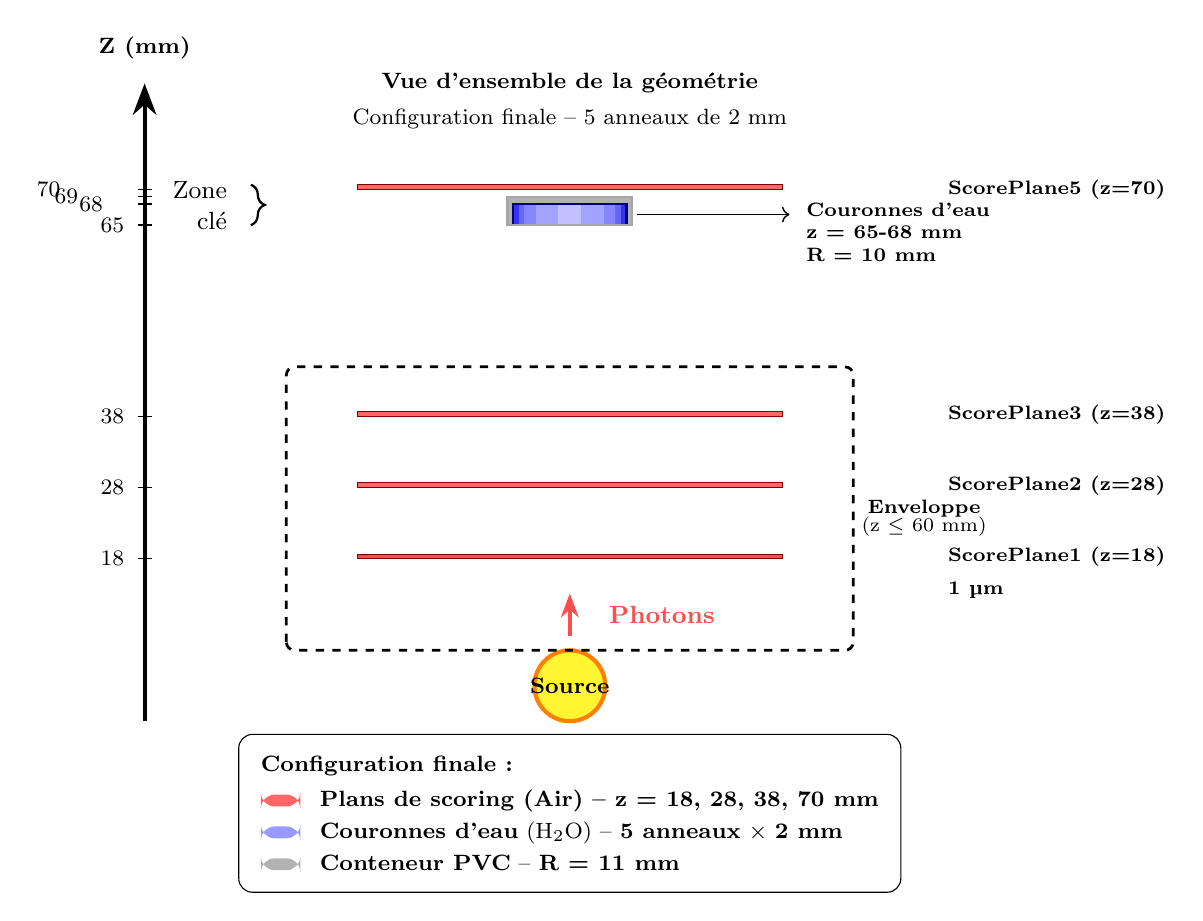
\begin{tikzpicture}[scale=0.9]

    % ============================================================
    % TITRE
    % ============================================================
    \node[font=\footnotesize\bfseries] at (6, 8.5) {Vue d'ensemble de la géométrie};
    \node[font=\footnotesize] at (6, 8.0) {Configuration finale -- 5 anneaux de 2 mm};

    % ============================================================
    % AXE Z PRINCIPAL (vertical)
    % ============================================================
    \draw[-{Stealth[length=4mm]}, line width=1.5pt] (0, -0.5) -- (0, 8.5);
    \node[font=\footnotesize\bfseries] at (0, 9) {\textbf{Z (mm)}};
    
    % ============================================================
    % SOURCE (en bas)
    % ============================================================
   \fill[yellow!80, draw=orange, line width=1.5pt] (6, 0) circle (0.5);
    \node[font=\footnotesize\bfseries] at (6, 0) {\textbf{Source}};
    \draw[-{Stealth[length=3mm]}, line width=1.5pt, red!70] (6, 0.7) -- (6, 1.3);
    \node[font=\small, red!70] at (7.3, 1.0) {\textbf{Photons}};
    
    % ============================================================
    % ENVELOPPE (boîte englobante ±60 mm)
    % ============================================================
    \draw[line width=1pt, dashed, black, rounded corners=3pt] (2, 0.5) rectangle (10, 4.5);
    \node[font=\scriptsize, black] at (11, 2.5) {\textbf{Enveloppe}};
    \node[font=\scriptsize, black] at (11, 2.25) {(z $\leq$ 60 mm)};
    
    % ============================================================
    % PLANS DE SCORING (dans l'enveloppe)
    % ============================================================
    
    % ScorePlane1 (z = 18 mm) - ultra fin
    \fill[red!70] (3, 1.8) rectangle (9, 1.85);
    \draw[line width=0.5pt, red!50!black] (3, 1.8) rectangle (9, 1.85);
    \node[font=\scriptsize, right] at (11.2, 1.82) {\textbf{ScorePlane1 (z=18)}};
    \node[font=\scriptsize, right, black] at (11.2, 1.35) {\textbf{1 µm}};
    
    % ScorePlane2 (z = 28 mm)
    \fill[red!60] (3, 2.8) rectangle (9, 2.87);
    \draw[line width=0.5pt, red!50!black] (3, 2.8) rectangle (9, 2.87);
    \node[font=\scriptsize, right] at (11.2, 2.83) {\textbf{ScorePlane2 (z=28)}};
    
    % ScorePlane3 (z = 38 mm)
    \fill[red!60] (3, 3.8) rectangle (9, 3.87);
    \draw[line width=0.5pt, red!50!black] (3, 3.8) rectangle (9, 3.87);
    \node[font=\scriptsize, right] at (11.2, 3.83) {\textbf{ScorePlane3 (z=38)}};
    
    % ============================================================
    % SYSTÈME DE COURONNES D'EAU (z = 65-69 mm) - 5 anneaux de 2 mm
    % ============================================================
    \def\waterY{6.5}
    \def\waterH{0.3}
    \def\pvcH{0.1}
    
    % Fond PVC (rayon total 11 mm)
    \fill[gray!60] (5.12, \waterY + \waterH) rectangle (6.88, \waterY + \waterH + \pvcH);
    
    % Parois PVC
    \fill[gray!60] (5.12, \waterY) rectangle (5.2, \waterY + 0.4);
    \fill[gray!60] (6.8, \waterY) rectangle (6.88, \waterY + 0.4);
    
    % Couronnes d'eau (vues de côté) - 5 anneaux de 2 mm
    % Couronne 0 (0-2 mm)
    \fill[blue!30, opacity=0.8] (5.84, \waterY) rectangle (6.16, \waterY + \waterH);
    % Couronne 1 (2-4 mm)
    \fill[blue!45, opacity=0.8] (5.52, \waterY) rectangle (5.84, \waterY + \waterH);
    \fill[blue!45, opacity=0.8] (6.16, \waterY) rectangle (6.48, \waterY + \waterH);
    % Couronne 2 (4-6 mm)
    \fill[blue!60, opacity=0.8] (5.36, \waterY) rectangle (5.52, \waterY + \waterH);
    \fill[blue!60, opacity=0.8] (6.48, \waterY) rectangle (6.64, \waterY + \waterH);
    % Couronne 3 (6-8 mm)
    \fill[blue!75, opacity=0.8] (5.28, \waterY) rectangle (5.36, \waterY + \waterH);
    \fill[blue!75, opacity=0.8] (6.64, \waterY) rectangle (6.72, \waterY + \waterH);
    % Couronne 4 (8-10 mm)
    \fill[blue!90!black, opacity=0.8] (5.2, \waterY) rectangle (5.28, \waterY + \waterH);
    \fill[blue!90!black, opacity=0.8] (6.72, \waterY) rectangle (6.8, \waterY + \waterH);
    
    % Contour
    \draw[line width=0.8pt, blue!50!black] (5.2, \waterY) rectangle (6.8, \waterY + \waterH);
    \draw[line width=0.8pt, gray!70] (5.12, \waterY) rectangle (6.88, \waterY + \waterH + \pvcH);
    
    % Annotation
    \node[font=\scriptsize, right, align=left] at (9.2, \waterY -0.1) {\textbf{Couronnes d'eau}\\\textbf{z = 65-68 mm}\\\textbf{R = 10 mm}};
    
    % Ligne de cote vers les couronnes
    \draw[line width=0.5pt, black, ->] (6.95, \waterY + 0.15) -- (9.1, \waterY + 0.15);
    
    % ============================================================
    % ScorePlane5 (z = 70 mm)
    % ============================================================
    \fill[red!60] (3, 7.0) rectangle (9, 7.07);
    \draw[line width=0.5pt, red!50!black] (3, 7.0) rectangle (9, 7.07);
    \node[font=\scriptsize, right] at (11.2, 7.) {\textbf{ScorePlane5 (z=70)}};
    
    % ============================================================
    % ANNOTATIONS Z SUR L'AXE
    % ============================================================
    \foreach \z/\label in {1.8/18, 2.8/28, 3.8/38} {
        \draw[line width=0.5pt] (-0.1, \z) -- (0.1, \z);
        \node[font=\footnotesize, left] at (-0.15, \z) {\label};
    }
    \draw[line width=0.5pt] (-0.1, 6.5) -- (0.1, 6.5);
    \node[font=\footnotesize, left] at (-0.15, 6.5) {65};
    \draw[line width=0.5pt] (-0.1, 6.8) -- (0.1, 6.8);
    \node[font=\footnotesize, left] at (-0.45, 6.8) {68};
    \draw[line width=0.5pt] (-0.1, 6.9) -- (0.1, 6.9);
    \node[font=\footnotesize, left] at (-0.80, 6.9) {69};
    \draw[line width=0.5pt] (-0.1, 7.0) -- (0.1, 7.0);
    \node[font=\footnotesize, left] at (-1.05, 7.0) {70};
    
    % Accolade pour zone d'intérêt
    \draw[decorate, decoration={brace, amplitude=5pt, mirror}, line width=0.8pt] 
        (1.5, 6.5) -- (1.5, 7.07);
    \node[font=\small, left, align=right] at (1.3, 6.78) {Zone\\clé};
    
    % ============================================================
    % LÉGENDE
    % ============================================================
    \node[draw, rectangle, rounded corners=5pt, fill=white, inner sep=8pt, font=\footnotesize, align=left] at (6, -1.8) {
        \footnotesize \textbf{Configuration finale :}\\[3pt]
        \tikz\fill[red!60] (0,0) rectangle (0.5,0.15); \, \footnotesize \textbf{Plans de scoring (Air) -- z = 18, 28, 38, 70 mm}\\[2pt]
        \tikz\fill[blue!50, opacity=0.8] (0,0) rectangle (0.5,0.15); \, \footnotesize \textbf{Couronnes d'eau} (H$_2$O) -- \textbf{5 anneaux} $\times$ \textbf{2 mm}\\[2pt]
        \tikz\fill[gray!60] (0,0) rectangle (0.5,0.15); \, \footnotesize \textbf{Conteneur PVC} -- \textbf{R = 11 mm}
    };

\end{tikzpicture}

\captionsetup{labelformat=empty}
\caption{\footnotesize \textit{Coupe longitudinale (plan $\bm{xz}$) de la géométrie Geant4. Le faisceau de rayons X est généré dans le tube X (gauche), traverse le collimateur en laiton, puis les six plans de scoring (P1--P6) avant d'atteindre la sphère d'eau cible.}}
\end{figure}

\noindent Six plans de scoring ont été positionnés perpendiculairement à l'axe de propagation du faisceau ($\bm{z}$) aux positions suivantes :\\

\begin{equation*}
z_i \in \{18, 28, 38, 118, 168\} \, \si{mm}
\end{equation*}

\noindent Les plans de scoring enregistrent les coordonnées d'impact $(\bm{x}, \bm{y})$ de chaque particule traversant le plan, ainsi que l'identifiant du parent (\texttt{parentID}) permettant de distinguer les particules primaires (\texttt{parentID = 0}) des particules secondaires (\texttt{parentID $\neq$ 0}).\\

%==============================================================================
\begin{figure}[H]
\centering
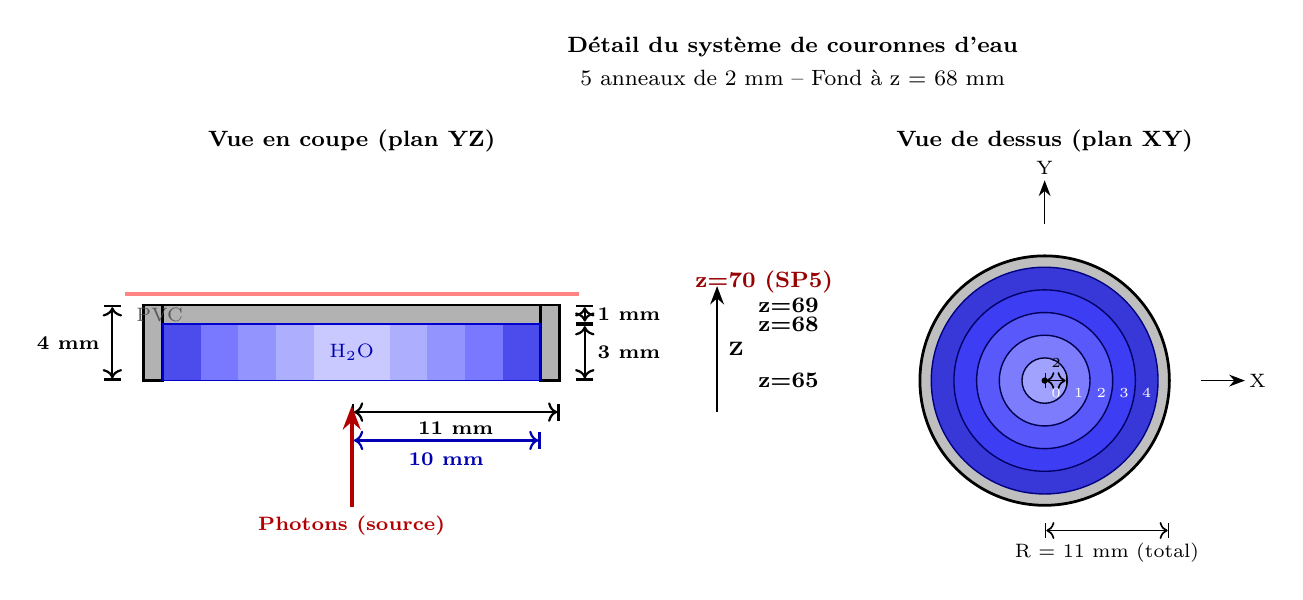
\begin{tikzpicture}[scale=0.8]

    % ============================================================
    % TITRE PRINCIPAL
    % ============================================================
    \node[font=\footnotesize\bfseries] at (4, 8.5) {Détail du système de couronnes d'eau};
    \node[font=\footnotesize] at (4, 8) {5 anneaux de 2 mm -- Fond à z = 68 mm};

    % ============================================================
    % VUE EN COUPE (gauche) - Plan YZ
    % ============================================================
    \node[font=\footnotesize\bfseries] at (-3, 7) {Vue en coupe (plan YZ)};
    
    % Échelle : 1 mm = 0.20 unités TikZ (plus grand car rayon plus petit)
    \def\scale{0.30}
    
    % Dimensions (en mm)
    \def\waterRadius{10}      % rayon eau = 10 mm (5 × 2 mm)
    \def\pvcThick{1}          % épaisseur PVC = 1 mm
    \def\waterThick{3}        % épaisseur eau = 3 mm
    \def\containerHeight{5}   % hauteur conteneur = 5 mm
    \def\wallHeight{4}        % hauteur parois = 4 mm
    
    % Position de référence (centre du système)
    \def\centerX{-3}
    \def\centerY{3.2}
    
    % Calcul des coordonnées
    \pgfmathsetmacro{\outerR}{(\waterRadius + \pvcThick) * \scale}
    \pgfmathsetmacro{\innerR}{\waterRadius * \scale}
    \pgfmathsetmacro{\waterH}{\waterThick * \scale}
    \pgfmathsetmacro{\pvcH}{\pvcThick * \scale}
    \pgfmathsetmacro{\wallH}{\wallHeight * \scale}
    
    % --- Fond PVC (gris) ---
    \fill[gray!60] (\centerX - \outerR, \centerY + \waterH) rectangle (\centerX + \outerR, \centerY + \waterH + \pvcH);
    \draw[line width=1pt, black] (\centerX - \outerR, \centerY + \waterH) rectangle (\centerX + \outerR, \centerY + \waterH + \pvcH);
    
    % --- Parois latérales PVC (gris) ---
    % Paroi gauche
    \fill[gray!60] (\centerX - \outerR, \centerY) rectangle (\centerX - \innerR, \centerY + \wallH);
    \draw[line width=1pt, black] (\centerX - \outerR, \centerY) rectangle (\centerX - \innerR, \centerY + \wallH);
    % Paroi droite
    \fill[gray!60] (\centerX + \innerR, \centerY) rectangle (\centerX + \outerR, \centerY + \wallH);
    \draw[line width=1pt, black] (\centerX + \innerR, \centerY) rectangle (\centerX + \outerR, \centerY + \wallH);
    
    % --- Couronnes d'eau (5 anneaux de 2 mm) ---
    % Couronne 4 (8-10 mm) - bleu foncé
    \fill[blue!90!black, opacity=0.7] (\centerX - 10*\scale, \centerY) rectangle (\centerX - 8*\scale, \centerY + \waterH);
    \fill[blue!90!black, opacity=0.7] (\centerX + 8*\scale, \centerY) rectangle (\centerX + 10*\scale, \centerY + \waterH);
    
    % Couronne 3 (6-8 mm)
    \fill[blue!75, opacity=0.7] (\centerX - 8*\scale, \centerY) rectangle (\centerX - 6*\scale, \centerY + \waterH);
    \fill[blue!75, opacity=0.7] (\centerX + 6*\scale, \centerY) rectangle (\centerX + 8*\scale, \centerY + \waterH);
    
    % Couronne 2 (4-6 mm)
    \fill[blue!60, opacity=0.7] (\centerX - 6*\scale, \centerY) rectangle (\centerX - 4*\scale, \centerY + \waterH);
    \fill[blue!60, opacity=0.7] (\centerX + 4*\scale, \centerY) rectangle (\centerX + 6*\scale, \centerY + \waterH);
    
    % Couronne 1 (2-4 mm)
    \fill[blue!45, opacity=0.7] (\centerX - 4*\scale, \centerY) rectangle (\centerX - 2*\scale, \centerY + \waterH);
    \fill[blue!45, opacity=0.7] (\centerX + 2*\scale, \centerY) rectangle (\centerX + 4*\scale, \centerY + \waterH);
    
    % Couronne 0 - disque central (0-2 mm) - bleu clair
    \fill[blue!30, opacity=0.7] (\centerX - 2*\scale, \centerY) rectangle (\centerX + 2*\scale, \centerY + \waterH);
    
    % Contour de l'eau
    \draw[line width=0.5pt, blue!80!black] (\centerX - \innerR, \centerY) rectangle (\centerX + \innerR, \centerY + \waterH);
    
    % --- Annotations avec cotes ---
    % Épaisseur eau
    \draw[|<->|, line width=0.8pt] (\centerX + \outerR + 0.4, \centerY) -- (\centerX + \outerR + 0.4, \centerY + \waterH);
    \node[font=\scriptsize, right] at (\centerX + \outerR + 0.45, \centerY + \waterH/2) {\textbf{3 mm}};
    
    % Épaisseur PVC fond
    \draw[|<->|, line width=0.8pt] (\centerX + \outerR + 0.4, \centerY + \waterH) -- (\centerX + \outerR + 0.4, \centerY + \waterH + \pvcH);
    \node[font=\scriptsize, right] at (\centerX + \outerR + 0.45, \centerY + \waterH + \pvcH/2) {\textbf{1 mm}};
    
    % Hauteur parois
    \draw[|<->|, line width=0.8pt] (\centerX - \outerR - 0.5, \centerY) -- (\centerX - \outerR - 0.5, \centerY + \wallH);
    \node[font=\scriptsize, left] at (\centerX - \outerR - 0.55, \centerY + \wallH/2) {\textbf{4 mm}};
    
    % Rayon total
    \draw[|<->|, line width=0.8pt] (\centerX, \centerY - 0.5) -- (\centerX + \outerR, \centerY - 0.5);
    \node[font=\scriptsize, below] at (\centerX + \outerR/2, \centerY - 0.5) {\textbf{11 mm}};
    
    % Rayon eau
    \draw[|<->|, line width=0.8pt, blue!70!black] (\centerX, \centerY - 0.95) -- (\centerX + \innerR, \centerY - 0.95);
    \node[font=\scriptsize, below, blue!70!black] at (\centerX + \innerR/2, \centerY - 1.0) {\textbf{10 mm}};
    
    % Flèche direction source
    \draw[-{Stealth[length=3mm]}, line width=1.5pt, red!70!black] (\centerX, \centerY - 2.0) -- (\centerX, \centerY - 0.4);
    \node[font=\scriptsize, red!70!black] at (\centerX, \centerY - 2.3) {\textbf{Photons (source)}};
    
    % Axe Z
    \draw[-{Stealth}, line width=0.8pt] (\centerX + \outerR + 2.5, \centerY - 0.5) -- (\centerX + \outerR + 2.5, \centerY + 1.5);
    \node[font=\scriptsize] at (\centerX + \outerR + 2.8, \centerY + 0.5) {\textbf{Z}};
    
    % Positions Z
    \node[font=\footnotesize, right] at (\centerX + \outerR + 3.0, \centerY) {\textbf{z=65}};
    \node[font=\footnotesize, right] at (\centerX + \outerR + 3.0, \centerY + \waterH) {\textbf{z=68}};
    \node[font=\footnotesize, right] at (\centerX + \outerR + 3.0, \centerY + \waterH + \pvcH) {\textbf{z=69}};
    
    % ScorePlane5 à z=70
    \fill[red!60, opacity=0.8] (\centerX - \outerR - 0.3, \centerY + \wallH + 0.15) rectangle (\centerX + \outerR + 0.3, \centerY + \wallH + 0.20);
    \node[font=\footnotesize, red!60!black, right] at (\centerX + \outerR + 2.0, \centerY + \wallH + 0.37) {\textbf{z=70 (SP5)}};
    
    % Labels matériaux
    \node[font=\scriptsize, gray!70!black] at (\centerX - \outerR + 0.25, \centerY + \wallH - 0.15) {PVC};
    \node[font=\scriptsize, blue!70!black] at (\centerX, \centerY + \waterH/2) {H$_2$O};

    % ============================================================
    % VUE DE DESSUS (droite) - Plan XY
    % ============================================================
    \node[font=\footnotesize\bfseries] at (8, 7) {Vue de dessus (plan XY)};
    
    \def\topCenterX{8}
    \def\topCenterY{3.2}
    \def\topScale{0.18}
    
    % Conteneur PVC (cercle extérieur)
    \fill[gray!50] (\topCenterX, \topCenterY) circle ({11*\topScale});
    \draw[line width=1pt, black] (\topCenterX, \topCenterY) circle ({11*\topScale});
    
    % Couronnes d'eau (du plus grand au plus petit)
    % Couronne 4 (8-10 mm)
    \fill[blue!90!black, opacity=0.7] (\topCenterX, \topCenterY) circle ({10*\topScale});
    \draw[line width=0.5pt, blue!50!black] (\topCenterX, \topCenterY) circle ({10*\topScale});
    
    % Couronne 3 (6-8 mm)
    \fill[blue!75, opacity=0.7] (\topCenterX, \topCenterY) circle ({8*\topScale});
    \draw[line width=0.5pt, blue!40!black] (\topCenterX, \topCenterY) circle ({8*\topScale});
    
    % Couronne 2 (4-6 mm)
    \fill[blue!60, opacity=0.7] (\topCenterX, \topCenterY) circle ({6*\topScale});
    \draw[line width=0.5pt, blue!35!black] (\topCenterX, \topCenterY) circle ({6*\topScale});
    
    % Couronne 1 (2-4 mm)
    \fill[blue!45, opacity=0.7] (\topCenterX, \topCenterY) circle ({4*\topScale});
    \draw[line width=0.5pt, blue!30!black] (\topCenterX, \topCenterY) circle ({4*\topScale});
    
    % Couronne 0 - disque central (0-2 mm)
    \fill[blue!30, opacity=0.7] (\topCenterX, \topCenterY) circle ({2*\topScale});
    \draw[line width=0.5pt, blue!20!black] (\topCenterX, \topCenterY) circle ({2*\topScale});
    
    % Centre
    \fill[black] (\topCenterX, \topCenterY) circle (0.05);
    
    % Annotations des rayons (ligne radiale avec dimensions)
    \draw[|<->|, line width=0.6pt] (\topCenterX, \topCenterY) -- (\topCenterX + 2*\topScale, \topCenterY);
    \node[font=\tiny, above] at (\topCenterX + 1*\topScale, \topCenterY + 0.05) {2};
    
    % Labels des couronnes
    \node[font=\tiny, white] at (\topCenterX + 1*\topScale, \topCenterY - 0.2) {0};
    \node[font=\tiny, white] at (\topCenterX + 3*\topScale, \topCenterY - 0.2) {1};
    \node[font=\tiny, white] at (\topCenterX + 5*\topScale, \topCenterY - 0.2) {2};
    \node[font=\tiny, white] at (\topCenterX + 7*\topScale, \topCenterY - 0.2) {3};
    \node[font=\tiny, white] at (\topCenterX + 9*\topScale, \topCenterY - 0.2) {4};
    
    % Cote rayon total
    \draw[|<->|, line width=0.6pt] (\topCenterX, \topCenterY - 11*\topScale - 0.4) -- (\topCenterX + 11*\topScale, \topCenterY - 11*\topScale - 0.4);
    \node[font=\scriptsize, below] at (\topCenterX + 5.5*\topScale, \topCenterY - 11*\topScale - 0.45) {R = 11 mm (total)};
    
    % Axes X et Y
    \draw[-{Stealth}, line width=0.6pt] (\topCenterX + 11*\topScale + 0.5, \topCenterY) -- (\topCenterX + 11*\topScale + 1.2, \topCenterY);
    \node[font=\scriptsize] at (\topCenterX + 11*\topScale + 1.4, \topCenterY) {X};
    \draw[-{Stealth}, line width=0.6pt] (\topCenterX, \topCenterY + 11*\topScale + 0.5) -- (\topCenterX, \topCenterY + 11*\topScale + 1.2);
    \node[font=\scriptsize] at (\topCenterX, \topCenterY + 11*\topScale + 1.4) {Y};

\end{tikzpicture}
\end{figure}

\noindent Le container est à la position $\bm{z}$  =68mm\\

%==============================================================================
\normalsize
\noindent \begin{mdframed}[backgroundcolor=orange!20]
\section{\Large \color{blue} \textbf{Source}\color{black}}
\end{mdframed}
\footnotesize
%==============================================================================

\begin{tcolorbox}[colback=blue!5,colframe=blue,title=\textbf{Configuration}]
\noindent Les figures suivantes montre les caractéristiques du spectre d'émission de la source utilisée:\\
${\rm \; \; \; \; \; \; }$ \textbf{-} \; La distribution de \color{blue}\textbf{l'énergie}\color{black} \; sous la forme du fond continu entre 3.5 keV et 50 keV\\
\noindent ${\rm \; \; \; \; \; \; }$ \textbf{-} \; La distribution de l'\color{blue}\textbf{angle $\bm{\theta}$}\color{black} \;  entre $\bm{\theta} = 0$ et $\bm{\theta} = 60$ degrés\\ 
\noindent ${\rm \; \; \; \; \; \; }$ \textbf{-} \; La distribution de \color{blue}\textbf{$\cos\bm{\theta}$}\color{black} \; uniforme entre $\cos\bm{0}$ et $\cos\bm{\pi/3}$\\
\noindent ${\rm \; \; \; \; \; \; }$ \textbf{-} \; La distribution de l'\color{blue}\textbf{angle $\bm{\phi}$}\color{black} \;  entre $\bm{\theta} = 0$ et $\bm{\theta} = 180$ degrés
\end{tcolorbox}

\begin{figure}[H]
\centering
\includegraphics[width=0.5\textwidth]{Figures/primary_gamma_energy.png}
\captionsetup{labelformat=empty}
\caption{\footnotesize \textit{Distribution énergie primaires}}
\end{figure}

\begin{figure}[H]
\centering
\includegraphics[width=0.5\textwidth]{Figures/primary_gamma_theta.png}
\captionsetup{labelformat=empty}
\caption{\footnotesize \textit{Distribution angle $\bm{\theta}$ primaire}}
\end{figure}

\begin{figure}[H]
\centering
\includegraphics[width=0.5\textwidth]{Figures/primary_gamma_costheta.png}
\captionsetup{labelformat=empty}
\caption{\footnotesize \textit{Distribution $\cos\bm{\theta}$ primaire}}
\end{figure}

\begin{figure}[H]
\centering
\includegraphics[width=0.6\textwidth]{Figures/primary_gamma_phi.png}
\captionsetup{labelformat=empty}
\caption{\footnotesize \textit{Distribution angle $\bm{\phi}$ primaire}}
\end{figure}

%==============================================================================
\normalsize
\noindent \begin{mdframed}[backgroundcolor=orange!20]
\section{\Large \color{blue} \textbf{Evaluation analytique du dépôt de dose}\color{black}\\[0.5em]
\large \color{blue} \textbf{pour 1000 photons $\gamma$ (4--50 keV) dans 3 mm d'eau}}
\end{mdframed}
\footnotesize
%==============================================================================

%===============================================================================
\normalsize
\noindent \begin{mdframed}[backgroundcolor=orange!20]
\subsection{\color{blue}\textbf{Sans collimation}\color{black}}
\end{mdframed}
\footnotesize
%===============================================================================
\medskip

% Couleurs personnalisées
\definecolor{water}{RGB}{64, 164, 223}
\definecolor{gamma}{RGB}{255, 193, 7}
\definecolor{dose1}{RGB}{255, 107, 107}
\definecolor{dose2}{RGB}{255, 160, 122}
\definecolor{dose3}{RGB}{255, 215, 0}
\definecolor{dose4}{RGB}{144, 238, 144}
\definecolor{dose5}{RGB}{135, 206, 235}

\begin{figure}[H]
\centering
\begin{tikzpicture}[scale=1.0]
    % Lame d'eau
    \fill[water!40] (0,0) rectangle (1.5,4);
    \draw[thick, water!80!black] (0,0) rectangle (1.5,4);
    
    % Hachures pour montrer l'extension infinie
    \foreach \y in {-0.3, 4.3} {
        \draw[dashed, gray] (-0.5,\y) -- (2,\y);
    }
    \node[black] at (0.75, 4.6) {\footnotesize \textbf{Extension infinie}};
    \node[black] at (0.75, -0.6) {\footnotesize \textbf{Extension infinie}};
    
    % Cotes
    \draw[<->, thick] (0,-1) -- (1.5,-1);
    \node[below] at (0.75,-1) {$\bm{x} = 3$ mm};
    
    \draw[<->, thick] (-0.5,0) -- (-0.5,4);
    \node[left, rotate=90] at (-0.7,2) {\footnotesize $\infty$};
    
    % Photons incidents
    \foreach \y in {0.5, 1.2, 1.8, 2.5, 3.2, 3.7} {
        \draw[-{Stealth[length=3mm]}, gamma!80!orange, very thick] (-2,\y) -- (-0.1,\y);
        \fill[gamma] (-2.2,\y) circle (0.1);
    }
    \node[left] at (-2.5, 2) {\footnotesize \textbf{1000 $\gamma$}};
    \node[left] at (-2.5, 1.3) {\footnotesize $\bm{E} \in [\bm{4}, \bm{50}]$ keV};
    
    % Interactions dans l'eau
    \foreach \pos in {(0.3,0.7), (0.8,1.5), (0.4,2.3), (1.1,3.0), (0.6,3.5)} {
        \node[star, star points=5, fill=red!70, inner sep=1pt] at \pos {};
    }
    
    % Légende
    \node[water!80!black, right] at (1.8, 3) {\textbf{Eau}};
    \node[right] at (1.8, 2.5) {\footnotesize $\bm{\rho} = 1$ g/cm$^3$};
    \node[red!70, right] at (1.8, 1.5) {\footnotesize $\star$ \textbf{Interactions}};
    
    % Photons transmis (atténués)
    \draw[-{Stealth[length=2mm]}, gamma!50, thick, dashed] (1.6,1.2) -- (3,1.2);
    \draw[-{Stealth[length=2mm]}, gamma!50, thick, dashed] (1.6,2.5) -- (3,2.5);
    \node[right, black] at (1.8, 1.85) {\footnotesize \textbf{Transmis}};
    
\end{tikzpicture}
\captionsetup{labelformat=empty}
\caption{\footnotesize \textit{Géométrie du problème : faisceau de photons $\gamma$ incident sur une lame d'eau de 3 mm d'épaisseur et d'extension latérale infinie.}}
\end{figure}

\noindent L'interaction des photons avec la matière est caractérisée par deux coefficients :
\begin{itemize}
\item $\bm{\mu}/\bm{\rho}$ : coefficient d'atténuation massique total (cm$^2$/g)
\item $\bm{\mu_{\text{en}}}/\bm{\rho}$ : coefficient d'absorption d'énergie massique (cm$^2$/g)
\end{itemize}

\begin{figure}[H]
\centering
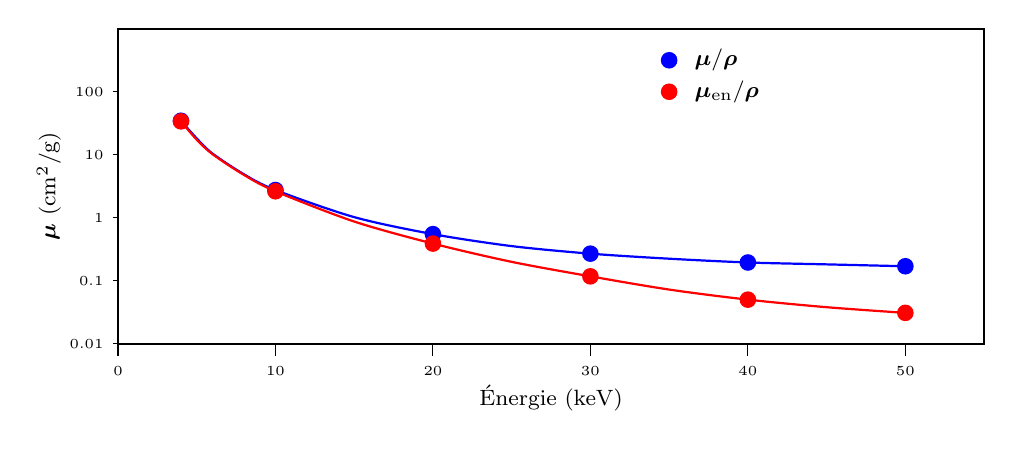
\begin{tikzpicture}[x=0.2cm, y=0.8cm]

    % Cadre
    \draw[thick] (0,0) rectangle (55,5);
    
    % Titre axes
    \node[below] at (27.5, -0.5) {\footnotesize Énergie (keV)};
    \node[rotate=90, above] at (-3, 2.5) {\footnotesize $\bm{\mu}$ (cm$^2$/g)};
    
    % Graduations X
    \foreach \x in {0, 10, 20, 30, 40, 50} {
        \draw (\x, 0) -- (\x, -0.2) node[below] {\tiny \x};
    }
    
    % Graduations Y (log: 0=0.01, 1=0.1, 2=1, 3=10, 4=100)
    \foreach \y/\val in {0/0.01, 1/0.1, 2/1, 3/10, 4/100} {
        \draw (0, \y) -- (-0.3, \y) node[left] {\tiny \val};
    }
    
    % μ/ρ (bleu) - valeurs: log10(μ)+2 pour ramener sur [0,5]
    \draw[blue, thick, smooth] plot coordinates {
        (4, 3.54) (5, 3.26) (6, 3.02) (8, 2.69) (10, 2.44)
        (15, 2.01) (20, 1.74) (25, 1.55) (30, 1.43)
        (35, 1.35) (40, 1.29) (45, 1.26) (50, 1.23)
    };
    \foreach \x/\y in {4/3.54, 10/2.44, 20/1.74, 30/1.43, 40/1.29, 50/1.23} {
        \fill[blue] (\x, \y) circle (3pt);
    }
    
    % μen/ρ (rouge)
    \draw[red, thick, smooth] plot coordinates {
        (4, 3.53) (5, 3.24) (6, 3.01) (8, 2.68) (10, 2.42)
        (15, 1.94) (20, 1.59) (25, 1.30) (30, 1.07)
        (35, 0.86) (40, 0.70) (45, 0.58) (50, 0.49)
    };
    \foreach \x/\y in {4/3.53, 10/2.42, 20/1.59, 30/1.07, 40/0.70, 50/0.49} {
        \fill[red] (\x, \y) circle (3pt);
    }
    
    % Légende
    \fill[blue] (35, 4.5) circle (3pt);
    \node[right] at (36, 4.5) {\footnotesize $\bm{\mu}/\bm{\rho}$};
    \fill[red] (35, 4.0) circle (3pt);
    \node[right] at (36, 4.0) {\footnotesize $\bm{\mu_{\text{en}}}/\bm{\rho}$};

\end{tikzpicture}
\captionsetup{labelformat=empty}
\caption{\footnotesize \textit{Coefficients d'atténuation massique de l'eau (échelle log, données NIST)}.}
\end{figure}

\noindent Pour un photon d'énergie $\bm{E}$, l'énergie moyenne déposée dans une épaisseur $\bm{x}$ de matériau est :

\begin{equation*}
\bm{E_{\text{dep}}}(\bm{E}) = \bm{E} \cdot \left(\bm{1} - e^{-\bm{\mu_{\text{en}}}(\bm{E}) \cdot \bm{\rho} \cdot \bm{x}}\right)
\end{equation*}

\noindent où :
\begin{itemize}
\item $\bm{\mu_{\text{en}}}(\bm{E})$ est le coefficient d'absorption d'énergie linéique (cm$^{-1}$)
\item $\bm{\rho}$ est la densité du matériau (g/cm$^3$)
\item $\bm{x}$ est l'épaisseur traversée (cm)
\end{itemize}

\noindent Pour un spectre de $\bm{N}$ photons avec une distribution en énergie $\bm{f(E)}$ :

\begin{equation*}
\bm{E_{\text{total}}} = \bm{N} \int_{\bm{E_{\min}}}^{\bm{E_{\max}}} \bm{E} \cdot \left(\bm{1} - e^{-\bm{\mu_{\text{en}}}(\bm{E}) \cdot \bm{\rho} \cdot \bm{x}}\right) \cdot \bm{f(E)} \, \bm{dE}
\end{equation*}

\noindent Pour une distribution uniforme : $\bm{f(E)} = \frac{\bm{1}}{\bm{E_{\max}} - \bm{E_{\min}}}$

\begin{equation*}
\bm{E_{\text{total}}} = 
\frac{\bm{N}}{\bm{E_{\max}} - \bm{E_{\min}}} \int_{4}^{50} \bm{E} \cdot \left(\bm{1} - e^{-\bm{\mu_{\text{en}}}\bm{(E)} \cdot \bm{\rho} \cdot \bm{x}}\right) \, \bm{dE}
\end{equation*}

\noindent La dose absorbée est définie comme l'énergie déposée par unité de masse :

\begin{equation*}
\bm{D} = \frac{\bm{E_{\text{total}}}}{\bm{m}} = \frac{\bm{E_{\text{total}}}}{\bm{\rho} \cdot \bm{x} \cdot \bm{S}}
\end{equation*}

\noindent Pour une surface $\bm{S} = 1$ cm$^2$ et nos paramètres :

\begin{align*}
\bm{D} &= \frac{\bm{2200} \text{ keV} \times \bm{1.602} \times \bm{10^{-16}} \text{ J/keV}}{0.3 \text{ g} \times 10^{-3} \text{ kg/g}} \\[1em]
&= \frac{\bm{3.52} \times \bm{10^{-13}} \text{ J}}{\bm{3} \times \bm{10^{-4}} \text{ kg}} \\[1em]
&= \bm{1.17} \times \bm{10^{-9}} \text{ Gy} = \bm{1.17} \text{ nGy}
\end{align*}

\begin{figure}[H]
\centering
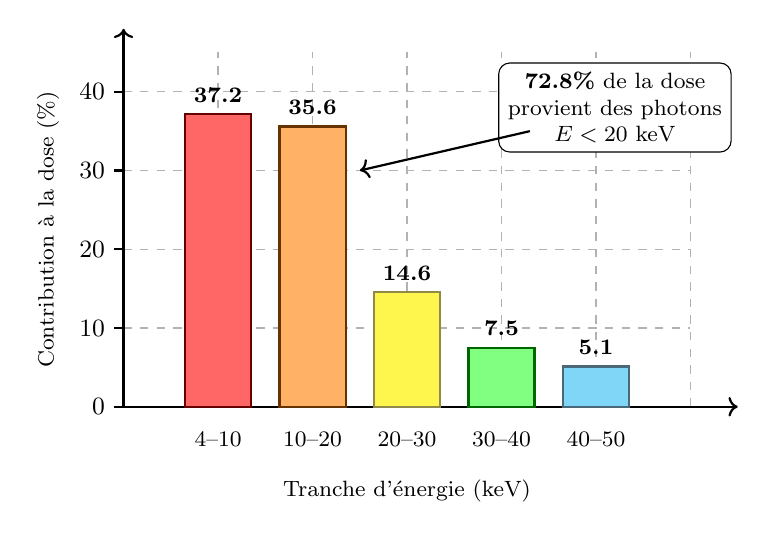
\begin{tikzpicture}[xscale=1.2, yscale=0.1]
    % Grille
    \draw[dashed, black!30] (0,0) grid[xstep=1, ystep=10] (6, 45);
    
    % Axes
    \draw[thick, ->] (0,0) -- (6.5,0);
    \draw[thick, ->] (0,0) -- (0,48);
    
    % Label axes
    \node[below] at (3, -8) {\footnotesize Tranche d'énergie (keV)};
    \node[rotate=90] at (-0.8, 22.5) {\footnotesize Contribution à la dose (\%)};
    
    % Graduations Y
    \foreach \y in {0, 10, 20, 30, 40} {
        \draw[thick] (-0.1, \y) -- (0, \y) node[left=3pt] {\small \y};
    }
    
    % Graduations X (labels des tranches)
    \foreach \x/\lab in {1/{4--10}, 2/{10--20}, 3/{20--30}, 4/{30--40}, 5/{40--50}} {
        \node[below] at (\x, -2) {\footnotesize \lab};
    }
    
    % Largeur des barres
    \def\bw{0.35}
    
    % Barre 1 : 37.2%
    \fill[red!60, draw=red!40!black, thick] (1-\bw, 0) rectangle (1+\bw, 37.2);
    \node[font=\footnotesize\bfseries] at (1, 39.5) {37.2};
    
    % Barre 2 : 35.6%
    \fill[orange!60, draw=orange!40!black, thick] (2-\bw, 0) rectangle (2+\bw, 35.6);
    \node[font=\footnotesize\bfseries] at (2, 38) {\footnotesize 35.6};
    
    % Barre 3 : 14.6%
    \fill[yellow!70, draw=yellow!50!black, thick] (3-\bw, 0) rectangle (3+\bw, 14.6);
    \node[font=\footnotesize\bfseries] at (3, 17) {\footnotesize 14.6};
    
    % Barre 4 : 7.5%
    \fill[green!50, draw=green!40!black, thick] (4-\bw, 0) rectangle (4+\bw, 7.5);
    \node[font=\footnotesize\bfseries] at (4, 10) {\footnotesize 7.5};
    
    % Barre 5 : 5.1%
    \fill[cyan!50, draw=cyan!40!black, thick] (5-\bw, 0) rectangle (5+\bw, 5.1);
    \node[font=\footnotesize\bfseries] at (5, 7.5) {\footnotesize 5.1};
    
    % Annotation
    \node[draw, fill=white, rounded corners, align=center, font=\footnotesize] at (5.2, 38) {
        \footnotesize \textbf{72.8\%} de la dose\\
        \footnotesize provient des photons\\
        \footnotesize $E < 20$ keV
    };
    \draw[->, thick] (4.3, 35) -- (2.5, 30);

\end{tikzpicture}
\captionsetup{labelformat=empty}
\caption{\footnotesize \textit{Contribution de chaque tranche d'énergie à la dose totale déposée. Les photons de basse énergie dominent malgré leur proportion uniforme dans le spectre incident}.}
\end{figure}

%===============================================================================
\normalsize
\noindent \begin{mdframed}[backgroundcolor=orange!20]
\subsection{\color{blue}\textbf{Avec collimation}\color{black}}
\end{mdframed}
\footnotesize
%===============================================================================
\medskip


%===============================================================================
\normalsize
\noindent \color{blue}\textbf{Efficacité du collimateur}\color{black}
\footnotesize
%===============================================================================
\medskip

\begin{tcolorbox}[colback=blue!5!white, colframe=blue!75!black, title=\textbf{Efficacité géométrique du collimateur}]
\begin{equation}
\varepsilon = \frac{N_{\text{transmis}}}{N_{\text{générés}}} = \frac{13\,695}{1\,000\,000} = \mathbf{1.37\%}
\end{equation}

\vspace{0.3cm}
\centering
\textbf{Soit environ 1 gamma sur 73 passe à travers le collimateur.}
\end{tcolorbox}

\clearpage

%===============================================================================
\normalsize
\noindent \color{blue}\textbf{Bilan des particules}\color{black}
\footnotesize
%===============================================================================
\medskip


\begin{figure}[H]
\centering
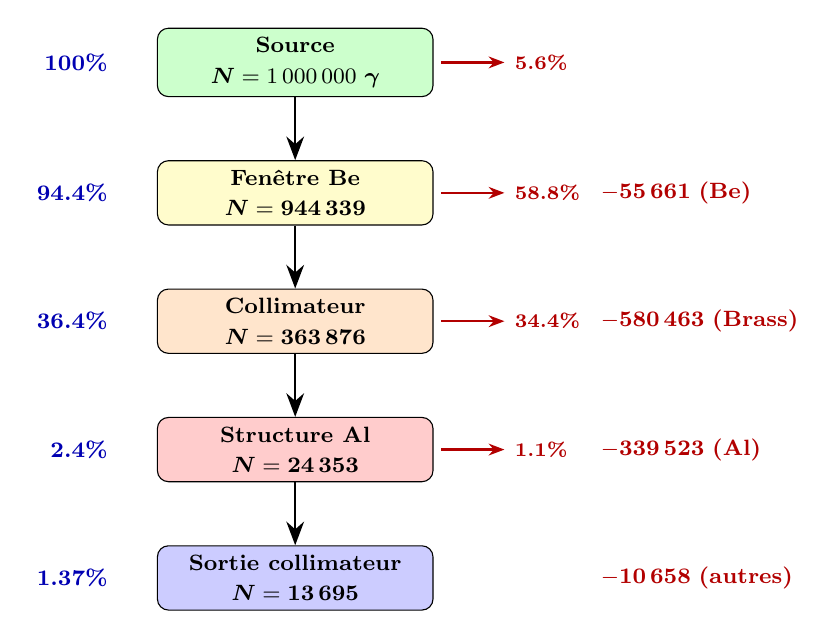
\begin{tikzpicture}[
    node distance=0.8cm,
    box/.style={rectangle, draw, rounded corners, minimum width=3.5cm, minimum height=0.8cm, align=center, font=\small},
    arrow/.style={-{Stealth[length=3mm]}, thick},
    loss/.style={-{Stealth[length=2mm]}, thick, red!70!black}
]
% Nœuds principaux
\node[box, fill=green!20] (source) {\footnotesize \textbf{Source}\\\footnotesize $\bm{N} = 1\,000\,000$ $\bm{\gamma}$};
\node[box, fill=yellow!20, below=of source] (be) {\footnotesize \textbf{Fenêtre Be}\\\footnotesize $\bm{N} = \bm{944\,339}$};
\node[box, fill=orange!20, below=of be] (coll) {\footnotesize \textbf{Collimateur}\\\footnotesize $\bm{N} = \bm{363\,876}$};
\node[box, fill=red!20, below=of coll] (al) {\footnotesize \textbf{Structure Al}\\\footnotesize $\bm{N} = \bm{24\,353}$};
\node[box, fill=blue!20, below=of al] (out) {\footnotesize \textbf{Sortie collimateur}\\\footnotesize $\bm{N} = \mathbf{13\,695}$};

% Flèches principales
\draw[arrow] (source) -- (be);
\draw[arrow] (be) -- (coll);
\draw[arrow] (coll) -- (al);
\draw[arrow] (al) -- (out);

% Pertes
\node[right=2cm of source, red!70!black, font=\footnotesize] (l0) {};
\node[right=2cm of be, red!70!black, font=\footnotesize] (l1) {$-\bm{55\,661}$ \textbf{(Be)}};
\node[right=2cm of coll, red!70!black, font=\footnotesize] (l2) {$-\bm{580\,463}$ \textbf{(Brass)}};
\node[right=2cm of al, red!70!black, font=\footnotesize] (l3) {$-\bm{339\,523}$ \textbf{(Al)}};
\node[right=2cm of out, red!70!black, font=\footnotesize] (l4) {$-\bm{10\,658}$ \textbf{(autres)}};

\draw[loss] (source.east) ++(0.1,0) -- ++(0.8,0) node[right, font=\scriptsize] {\textbf{5.6\%}};
\draw[loss] (be.east) ++(0.1,0) -- ++(0.8,0) node[right, font=\scriptsize] {\textbf{58.8\%}};
\draw[loss] (coll.east) ++(0.1,0) -- ++(0.8,0) node[right, font=\scriptsize] {\textbf{34.4\%}};
\draw[loss] (al.east) ++(0.1,0) -- ++(0.8,0) node[right, font=\scriptsize] {\textbf{1.1\%}};

% Pourcentages à gauche
\node[left=0.5cm of source, font=\footnotesize, blue!70!black] {\textbf{100\%}};
\node[left=0.5cm of be, font=\footnotesize, blue!70!black] {\textbf{94.4\%}};
\node[left=0.5cm of coll, font=\footnotesize, blue!70!black] {\textbf{36.4\%}};
\node[left=0.5cm of al, font=\footnotesize, blue!70!black] {\textbf{2.4\%}};  
\node[left=0.5cm of out, font=\footnotesize, blue!70!black] {\textbf{1.37\%}};
\end{tikzpicture}
\captionsetup{labelformat=empty}
\caption{\footnotesize \textit{Diagramme de flux des photons à travers le système de collimation. Les pertes par absorption photoélectrique sont indiquées en rouge}.}
\end{figure}

%===============================================================================
\normalsize
\noindent \color{blue}\textbf{Répartition des absorptions par matériau}\color{black}
\footnotesize
%===============================================================================
\medskip
  
\begin{table}[H]
\centering
\begin{tabular}{lrrr}
\toprule
\footnotesize \textbf{Matériau}&\footnotesize \textbf{Photons absorbés}&\footnotesize \textbf{Pourcentage}&\footnotesize \textbf{Rôle} \\
\midrule
\rowcolor{orange!20} \footnotesize Laiton (Brass)&\footnotesize \num{580463}&\footnotesize 58.8\% &\footnotesize Collimateur\\
\rowcolor{gray!15} \footnotesize Aluminium&\footnotesize \num{339523}&\footnotesize 34.4\%&\footnotesize Structure/support\\
\rowcolor{cyan!15} \footnotesize Béryllium&\footnotesize \num{55661}&\footnotesize 5.6\%&\footnotesize Fenêtre de sortie\\
\footnotesize Air&\footnotesize \num{7475}&\footnotesize 0.8\%&\footnotesize Milieu ambiant \\
\footnotesize Tungstene&\footnotesize \num{1538}&\footnotesize 0.2\% &\footnotesize Anode \\
\footnotesize Al$_2$O $_3$&\footnotesize \num{1363}&\footnotesize 0.1\% &\footnotesize Isolant \\
\footnotesize Acier Inox 304 &\footnotesize \num{1249}&\footnotesize 0.1\%&\footnotesize Enveloppe \\
\midrule
\footnotesize \textbf{Total absorbés} &\footnotesize \textbf{\num{987272}} &\footnotesize \textbf{98.7\%} & \\
\rowcolor{green!20} \footnotesize \textbf{Transmis} &\footnotesize \textbf{\num{13695}} &\footnotesize \textbf{1.37\%} &\footnotesize \textbf{Faisceau utile} \\
\bottomrule
\end{tabular}
\captionsetup{labelformat=empty}
\caption{\footnotesize \textit{Répartition des photons absorbés par matériau. Le processus dominant est l'effet photoélectrique}.}
\end{table}

%===============================================================================
\normalsize
\noindent \color{blue}\textbf{Analyse de la transmission}\color{black}
\footnotesize
%===============================================================================
\medskip

\noindent L'efficacité du collimateur peut être définie de plusieurs façons :

\begin{enumerate}
\item \textbf{Efficacité globale} (par rapport aux photons générés) :
\begin{equation*}
\bm{\varepsilon_{\text{global}}} = \frac{\bm{N_{\text{transmis}}}}{\bm{N_{\text{générés}}}} = \frac{\bm{13\,695}}{\bm{1\,000\,000}} = \bm{1.37}\%
\end{equation*}

\item \textbf{Efficacité géométrique} (par rapport aux photons sortis du Be) :

\begin{equation*}
\bm{\varepsilon_{\text{géom}}} = \frac{\bm{N_{\text{transmis}}}}{\bm{N_{\text{sortis Be}}}} = \frac{\bm{13\,695}}{\bm{944\,339}} = \bm{1.45}\%
\end{equation*}

\item \textbf{Rapport de collimation} :
\begin{equation*}
\bm{R} = \frac{\bm{1}}{\bm{\varepsilon_{\text{global}}}} \approx \bm{73}
\end{equation*}
\end{enumerate}

\begin{tcolorbox}[colback=blue!5!white, colframe=blue!75!black, title=\textbf{Efficacité géométrique du collimateur}]
\begin{itemize}
\item Le collimateur en \textbf{laiton} joue son rôle principal d'absorbeur : il arrête \textbf{59\%} des photons émis par la source.
\item La \textbf{structure en aluminium} contribue également de manière significative à l'atténuation (34\%).
\item La \textbf{fenêtre en béryllium} est relativement transparente aux rayons X (seulement 5.6\% d'absorption), ce qui est attendu pour ce matériau à faible $Z$.
\item L'ouverture effective du collimateur ne laisse passer que \textbf{1.37\%} du flux initial.
\end{itemize}
\end{tcolorbox}

%===============================================================================
\normalsize
\noindent \color{blue}\textbf{Dosimétrie dans l'eau}\color{black}
\footnotesize
%===============================================================================
\medskip

\noindent Pour \num{1000000} photons émis par la source, la  dose totale déposée est :

\begin{table}[H]
\centering
\begin{tabular}{ll}
\toprule
\footnotesize \textbf{Grandeur} & \footnotesize \textbf{Valeur} \\
\midrule
\footnotesize Énergie totale déposée &\footnotesize \SI{64130.3}{keV} \\
\footnotesize Dose totale dans l'eau &\footnotesize \SI{10.90}{nGy} \\
\footnotesize Photons atteignant l'eau &\footnotesize $\sim 13\,500$ \\
\footnotesize Dose par photon transmis &\footnotesize $\sim \SI{0.8}{pGy/\gamma}$ \\
\bottomrule
\end{tabular}
\captionsetup{labelformat=empty}
\caption{\footnotesize \textit{Bilan dosimétrique pour \num{1000000} photons primaires}.}
\end{table}


\begin{table}[H]
\centering
\begin{tabular}{ccccc}
\toprule
\footnotesize \textbf{Anneau}&\footnotesize\textbf{Rayon (mm)}&\footnotesize \textbf{Énergie (keV)}&\footnotesize \textbf{Dose (nGy)}&\footnotesize \textbf{Fraction}\\
\midrule
\footnotesize 0&\footnotesize 0--2&\footnotesize \num{3626.8}&\footnotesize 15.41&\footnotesize 23.3\%\\
\footnotesize 1&\footnotesize 2--4&\footnotesize \num{11801.8}&\footnotesize 16.72&\footnotesize 25.3\%\\
\footnotesize 2&\footnotesize 4--6&\footnotesize \num{20382.0}&\footnotesize 17.32&\footnotesize 26.2\%\\
\footnotesize 3&\footnotesize 6--8&\footnotesize \num{26841.7}&\footnotesize 16.29&\footnotesize 24.6\%\\
\footnotesize 4&\footnotesize 8--10&\footnotesize \num{1478.0}&\footnotesize 0.70&\footnotesize 1.1\%\\
\midrule
\footnotesize \textbf{Total}&\footnotesize 0--10&\footnotesize \textbf{\num{64130.3}}&\footnotesize \textbf{10.90}$^*$&\footnotesize  100\% \\
\bottomrule
\end{tabular}
\captionsetup{labelformat=empty}
\caption{\footnotesize \textit{Distribution de la dose par anneau concentrique dans l'eau. $^*$La dose totale est la moyenne pondérée par les masses}.}
\end{table}

\begin{figure}[H]
\centering
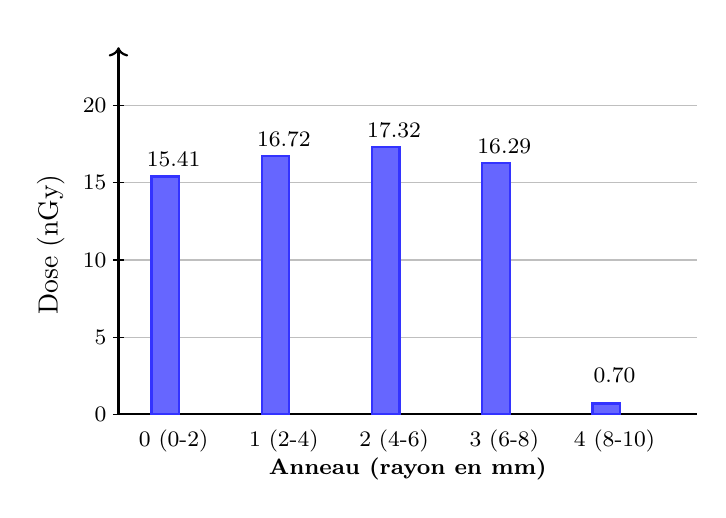
\begin{tikzpicture}[scale=0.7]
    % Paramètres
    \def\largeurBarre{0.5}    % largeur des barres en cm
    \def\echelle{0.28}       % échelle verticale (cm par nGy)
    \def\espacement{1.0}      % espacement entre les barres en cm
    \def\ymax{22}             % valeur max de l'axe Y
    
    % Données: {position, valeur, label}
    \def\données{
        {0, 15.41, 0 (0-2)},
        {1, 16.72, 1 (2-4)},
        {2, 17.32, 2 (4-6)},
        {3, 16.29, 3 (6-8)},
        {4, 0.70, 4 (8-10)}
    }
    
    % Axe Y
    \draw[thick, ->] (0,0) -- (0, \ymax*\echelle + 0.5) node[above] {};
    \node[rotate=90, anchor=south] at (-0.8, \ymax*\echelle/2) {Dose (nGy)};
    
    % Graduations Y
    \foreach \y in {0, 5, 10, 15, 20} {
        \draw[gray!50] (0, \y*\echelle) -- (10.5, \y*\echelle);
        \draw (-0.1, \y*\echelle) -- (0.1, \y*\echelle) node[left, xshift=-0.1cm] {\footnotesize \y};
    }
    
    % Axe X
    \draw[thick] (0,0) -- (10.5, 0);
    \node at (5.25, -1.0) {\footnotesize \textbf{Anneau (rayon en mm)}};
    
    % Barres et labels
    % Anneau 0
    \fill[blue!60] (0.6, 0) rectangle +(\largeurBarre, 15.41*\echelle);
    \draw[blue!80, thick] (0.6, 0) rectangle +(\largeurBarre, 15.41*\echelle);
    \node[above, font=\footnotesize] at (1, 15.41*\echelle) {15.41};
    \node[below, font=\footnotesize] at (1, -0.1) {0 (0-2)};
    
    % Anneau 1
    \fill[blue!60] (2.6, 0) rectangle +(\largeurBarre, 16.72*\echelle);
    \draw[blue!80, thick] (2.6, 0) rectangle +(\largeurBarre, 16.72*\echelle);
    \node[above, font=\footnotesize] at (3, 16.72*\echelle) {16.72};
    \node[below, font=\footnotesize] at (3, -0.1) {1 (2-4)};
    
    % Anneau 2
    \fill[blue!60] (4.6, 0) rectangle +(\largeurBarre, 17.32*\echelle);
    \draw[blue!80, thick] (4.6, 0) rectangle +(\largeurBarre, 17.32*\echelle);
    \node[above, font=\footnotesize] at (5, 17.32*\echelle) {17.32};
    \node[below, font=\footnotesize] at (5, -0.1) {2 (4-6)};
    
    % Anneau 3
    \fill[blue!60] (6.6, 0) rectangle +(\largeurBarre, 16.29*\echelle);
    \draw[blue!80, thick] (6.6, 0) rectangle +(\largeurBarre, 16.29*\echelle);
    \node[above, font=\footnotesize] at (7, 16.29*\echelle) {16.29};
    \node[below, font=\footnotesize] at (7, -0.1) {3 (6-8)};
    
    % Anneau 4
    \fill[blue!60] (8.6, 0) rectangle +(\largeurBarre, 0.70*\echelle);
    \draw[blue!80, thick] (8.6, 0) rectangle +(\largeurBarre, 0.70*\echelle);
    \node[above, font=\footnotesize] at (9, 0.70*\echelle + 0.2) {0.70};
    \node[below, font=\footnotesize] at (9, -0.1) {4 (8-10)};
    
\end{tikzpicture}
\captionsetup{labelformat=empty}
\caption{\footnotesize \textit{Distribution radiale de la dose dans les anneaux d'eau ($\bm{r}$ en mm)}.}
\end{figure}

\clearpage

%===============================================================================
\normalsize
\noindent \color{blue}\textbf{Conclusion}\color{black}
\footnotesize
%===============================================================================
\medskip

\begin{tcolorbox}[colback=blue!5!white, colframe=blue!75!black, title=\textbf{Efficacité géométrique du collimateur}]
\noindent $\bullet$ Avec le calcul analytique, pour \num{1000000} photons émis par la source, la  dose totale déposée est :
\begin{equation*}
\bm{D} = 1000 \times \bm{1.17} \text{ nGy} = \bm{1170} \text{ nGy}
\end{equation*}
\noindent $\bullet$ Si on applique le facteur d'efficacité de $\bm{1.34}\%$, la  dose totale déposée est :
\begin{equation*}
\bm{D} =  \bm{1170} \times \bm{0.0134} = 15.67 \text{ nGy}
\end{equation*}
\noindent $\bullet$ à comparer avec la valeur simulée de $\bm{15.67} \text{ nGy}$
\end{tcolorbox}

\clearpage

%==============================================================================
\normalsize
\noindent \begin{mdframed}[backgroundcolor=orange!20]
\section{\Large \color{blue} \textbf{Ntuples (TTrees) et Histogrammes}\color{black}}
\end{mdframed}
\footnotesize
%==============================================================================


\noindent Le fichier \color{blue}\textbf{output.root}\color{black} \; contient :
\begin{itemize}
\item \color{blue}\textbf{15 histogrammes 1D}\color{black} (H0--H14) pour les distributions d'énergie et de dose
\item \color{blue}\textbf{5 ntuples}\color{black} pour les données particule par particule aux différents plans de mesure
\end{itemize}

\begin{table}[H]
\centering
\captionsetup{labelformat=empty}
\caption{\footnotesize \textit{Liste des histogrammes 1D}}
\begin{tabular}{@{}clllc@{}}
\toprule
\rowcolor{header!20} \footnotesize \textbf{ID} &\footnotesize \textbf{Nom} &\footnotesize \textbf{Description} &\footnotesize \textbf{Unité} &\footnotesize \textbf{Bins} \\
\midrule
\rowcolor{lightgray}
\footnotesize H0 &\footnotesize \texttt{E\_emission} &\footnotesize Énergie des gammas à l'émission &\footnotesize keV &\footnotesize 150 \\
\footnotesize H1 &\footnotesize \texttt{theta\_emission} &\footnotesize Angle $\theta$ à l'émission &\footnotesize degrés &\footnotesize 180 \\
\rowcolor{lightgray}
\footnotesize H2 &\footnotesize \texttt{phi\_emission} &\footnotesize Angle $\phi$ à l'émission &\footnotesize degrés &\footnotesize 90 \\
\footnotesize H3 &\footnotesize \texttt{Dose\_total\_run} &\footnotesize Dose totale (run complet) &\footnotesize pGy &\footnotesize 1000 \\
\rowcolor{lightgray}
\footnotesize H4 &\footnotesize \texttt{Dose\_total\_10000evt} &\footnotesize Dose totale (par 10000 evt) &\footnotesize pGy &\footnotesize 200 \\
\footnotesize H5--H9 &\footnotesize \texttt{Dose\_ring*\_run} &\footnotesize Dose par anneau (run) &\footnotesize pGy &\footnotesize 1000 \\
\rowcolor{lightgray}
\footnotesize H10--H14 &\footnotesize \texttt{Dose\_ring*\_10000evt} &\footnotesize Dose par anneau (10000 evt) &\footnotesize pGy &\footnotesize 200 \\
\bottomrule
\end{tabular}
\end{table}

\begin{table}[H]
\centering
\captionsetup{labelformat=empty}
\caption{\footnotesize Liste des ntuples}
\begin{tabular}{@{}clcc@{}}
\toprule
\rowcolor{header!20} \footnotesize \textbf{ID} &\footnotesize  \textbf{Nom} &\footnotesize  \textbf{Position $z$} &\footnotesize  \textbf{Détecteur} \\
\midrule
\rowcolor{lightgray}
\footnotesize 0 &\footnotesize  \texttt{plane\_passages} &\footnotesize  18 mm &\footnotesize  SurfaceSpectrumSD (SpecSD) \\
\footnotesize 1 &\footnotesize  \texttt{ScorePlane2\_passages} &\footnotesize  28 mm &\footnotesize  ScorePlane2SD \\
\rowcolor{lightgray}
\footnotesize 2 &\footnotesize  \texttt{ScorePlane3\_passages} &\footnotesize  38 mm &\footnotesize  ScorePlane3SD \\
\footnotesize 3 &\footnotesize  \texttt{WaterRings\_passages} &\footnotesize  65--68 mm &\footnotesize  ScorePlane4SD \\
\rowcolor{lightgray}
\footnotesize 4 &\footnotesize  \texttt{ScorePlane5\_passages} &\footnotesize  70 mm &\footnotesize  ScorePlane5SD \\
\bottomrule
\end{tabular}
\end{table}

\noindent Tous les ntuples partagent la même structure de colonnes :

\begin{table}[H]
\centering
\captionsetup{labelformat=empty}
\caption{\footnotesize \textit{Colonnes des ntuples}}
\begin{tabular}{@{}clll@{}}
\toprule
\rowcolor{header!20} \footnotesize \textbf{Col.} &\footnotesize  \textbf{Nom} &\footnotesize  \textbf{Type} &\footnotesize  \textbf{Description} \\
\midrule
\rowcolor{lightgray}
\footnotesize 0 &\footnotesize  \texttt{pdg} &\footnotesize  \texttt{int} &\footnotesize  Code PDG de la particule \\
\footnotesize 1 &\footnotesize  \texttt{name} &\footnotesize  \texttt{string} &\footnotesize  Nom de la particule \\
\rowcolor{lightgray}
\footnotesize 2 &\footnotesize  \texttt{is\_secondary} &\footnotesize  \texttt{int} &\footnotesize  0 = primaire, 1 = secondaire \\
\footnotesize 3 &\footnotesize  \texttt{x\_mm} &\footnotesize  \texttt{double} &\footnotesize  Position $x$ (mm) \\
\rowcolor{lightgray}
\footnotesize 4 &\footnotesize  \texttt{y\_mm} &\footnotesize  \texttt{double} &\footnotesize  Position $y$ (mm) \\
\footnotesize 5 &\footnotesize  \texttt{ekin\_keV} &\footnotesize  \texttt{double} &\footnotesize  Énergie cinétique (keV) \\
\rowcolor{lightgray}
\footnotesize 6 &\footnotesize  \texttt{trackID} &\footnotesize  \texttt{int} &\footnotesize  Identifiant du track \\
\footnotesize 7 &\footnotesize  \texttt{parentID} & \footnotesize \texttt{int} &\footnotesize  ID du parent (0 si primaire) \\
\rowcolor{lightgray}
\footnotesize 8 &\footnotesize  \texttt{creator\_process} &\footnotesize  \texttt{string} &\footnotesize  Processus créateur \\
\bottomrule
\end{tabular}
\end{table}

\noindent \textbf{Note :} Le ntuple \textbf{plane\_passages} (ID 0) possède une colonne supplémentaire :
\begin{itemize}
 \item Colonne 5 : \texttt{z\_mm} (position $z$ en mm)
\item Les colonnes suivantes sont décalées d'un index
\end{itemize}
%===============================================================================
\normalsize
\noindent \begin{mdframed}[backgroundcolor=orange!20]
\subsection{\color{blue}\textbf{Histogrammes d'émission (H0--H2)}\color{black}}
\end{mdframed}
\footnotesize
%===============================================================================
\medskip

\noindent Ces histogrammes caractérisent les particules primaires au moment de leur génération.
\medskip

%===============================================================================
\normalsize
\noindent \color{blue}\textbf{H0 : Énergie à l'émission}\color{black}
\footnotesize
%===============================================================================

\begin{table}[H]
\centering
\begin{tabular}{@{}ll@{}}
\toprule
\rowcolor{header!20} \footnotesize \textbf{Paramètre} &\footnotesize \textbf{Valeur} \\
\midrule
\footnotesize Nom ROOT &\footnotesize \texttt{E\_emission} \\
\footnotesize Plage &\footnotesize $[0, 50]$ keV \\
\footnotesize Nombre de bins & 150 \\
\footnotesize Fichier source &\footnotesize \texttt{PrimaryGeneratorAction2.cc} \\
\footnotesize Ligne de code &\footnotesize \texttt{man->FillH1(0, energy);} \\
\bottomrule
\end{tabular}
\end{table}

\begin{itemize}
\item Appelé dans \texttt{GeneratePrimaries()} après tirage de l'énergie
\item Uniquement si $E > 3.5$ keV (coupure basse énergie)
\item Distribution tabulée du spectre de rayons X (tungstène, 50 kVp)
\end{itemize}

%===============================================================================
\normalsize
\noindent \color{blue}\textbf{H1 : Angle polaire $\theta$}\color{black}
\footnotesize
%===============================================================================

\begin{table}[H]
\centering
\begin{tabular}{@{}ll@{}}
\toprule
\rowcolor{header!20} \footnotesize \textbf{Paramètre} &\footnotesize \textbf{Valeur} \\
\midrule
\footnotesize Nom ROOT &\footnotesize \texttt{theta\_emission} \\
\footnotesize Plage &\footnotesize $[0, 180]$ degrés \\
\footnotesize Nombre de bins &\footnotesize 180 \\
\footnotesize Fichier source &\footnotesize \texttt{PrimaryGeneratorAction2.cc} \\
\footnotesize Ligne de code &\footnotesize  \texttt{man->FillH1(1, alphaDeg);} \\
\bottomrule
\end{tabular}
\end{table}

\begin{itemize}
\item Angle $\theta$ tiré uniformément dans un cône de demi-angle 60°
\item $\cos\theta \in [\cos(60°), \cos(0°)] = [0.5, 1.0]$
\end{itemize}

%===============================================================================
\normalsize
\noindent \color{blue}\textbf{H2 : Angle azimutal $\phi$}\color{black}
\footnotesize
%===============================================================================

\begin{table}[H]
\centering
\begin{tabular}{@{}ll@{}}
\toprule
\rowcolor{header!20} \footnotesize \textbf{Paramètre} &\footnotesize \textbf{Valeur} \\
\midrule
\footnotesize Nom ROOT &\footnotesize \texttt{phi\_emission} \\
\footnotesize Plage &\footnotesize $[-180, 180]$ degrés \\
\footnotesize Nombre de bins &\footnotesize 90 \\
\footnotesize Fichier source &\footnotesize \texttt{PrimaryGeneratorAction2.cc} \\
\footnotesize Ligne de code &\footnotesize \texttt{man->FillH1(2, psiDeg);} \\
\bottomrule
\end{tabular}
\end{table}

\begin{itemize}
\item Angle $\phi$ tiré uniformément dans $[0°, 360°]$
\end{itemize}

%===============================================================================
\normalsize
\noindent \begin{mdframed}[backgroundcolor=orange!20]
\subsection{\color{blue}\textbf{Histogrammes de dose (H3--H14)}\color{black}}
\end{mdframed}
\footnotesize
%===============================================================================
\medskip

\noindent La dose est calculée selon :
\begin{equation*}
\bm{D} \text{ [pGy]} = \bm{E_{\text{dep}}} \text{ [keV]} \times \frac{\bm{0.1602}}{\bm{m} \text{ [g]}}
\end{equation*}

\noindent où le facteur de conversion vient de :
\begin{align*}
1 \text{ keV} &= \bm{1.602} \times \bm{10^{-16}} \text{ J} \\
1 \text{ Gy} &= 1 \text{ J/kg} = \bm{10^{12}} \text{ pGy}
\end{align*}

\begin{table}[H]
\centering
\captionsetup{labelformat=empty}
\caption{\footnotesize Géométrie et masses des anneaux d'eau (épaisseur 3 mm, $\bm{\rho }= 1$ g/cm$^3$)}
\begin{tabular}{@{}ccccc@{}}
\toprule
\rowcolor{header!20}\footnotesize\textbf{Anneau} &\footnotesize \textbf{Rayon} &\footnotesize \textbf{Volume} &\footnotesize \textbf{Masse} &\footnotesize \textbf{Constante} \\
\rowcolor{header!20} &\footnotesize (mm) &\footnotesize (mm$^3$) &\footnotesize (g) & \\
\midrule
\footnotesize 0 &\footnotesize 0--2 &\footnotesize $\pi \times 4 \times 3$ &\footnotesize 0.0377 &\footnotesize \texttt{kMassRing[0]} \\
\footnotesize 1 &\footnotesize 2--4 &\footnotesize $\pi \times 12 \times 3$ &\footnotesize 0.1131 &\footnotesize \texttt{kMassRing[1]} \\
\footnotesize 2 &\footnotesize 4--6 &\footnotesize $\pi \times 20 \times 3$ &\footnotesize 0.1885 &\footnotesize \texttt{kMassRing[2]} \\
\footnotesize 3 &\footnotesize 6--8 &\footnotesize $\pi \times 28 \times 3$ &\footnotesize 0.2639 &\footnotesize \texttt{kMassRing[3]} \\
\footnotesize 4 &\footnotesize 8--10 &\footnotesize $\pi \times 36 \times 3$ &\footnotesize 0.3393 &\footnotesize \texttt{kMassRing[4]} \\
\midrule
\footnotesize \textbf{Total} &\footnotesize 0--10 &\footnotesize $\pi \times 100 \times 3$ &\footnotesize 0.9425 &\footnotesize \texttt{kMassTotalWater} \\
\bottomrule
\end{tabular}
\end{table}

%===============================================================================
\normalsize
\noindent \color{blue}\textbf{H3 : Dose totale du run}\color{black}
\footnotesize
%===============================================================================

\begin{table}[H]
\centering
\begin{tabular}{@{}ll@{}}
\toprule
\rowcolor{header!20} \footnotesize \textbf{Paramètre} &\footnotesize \textbf{Valeur} \\
\midrule
\footnotesize Nom ROOT &\footnotesize \texttt{Dose\_total\_run} \\
\footnotesize Plage &\footnotesize $[0, 5\,000\,000]$ pGy \\
\footnotesize Fichier source &\footnotesize \texttt{RunAction.cc} (EndOfRunAction) \\
\footnotesize Ligne de code &\footnotesize \texttt{am->FillH1(3, dose\_total\_run\_pGy);} \\
\bottomrule
\end{tabular}
\end{table}

\begin{itemize}
\item Rempli \textbf{une seule fois} à la fin du run
\item Valeur = dose cumulée sur tous les événements
\item Plage étendue pour supporter jusqu'à 500M événements
\end{itemize}

%===============================================================================
\normalsize
\noindent \color{blue}\textbf{H4 : Dose totale par 10000 événements}\color{black}
\footnotesize
%===============================================================================

\begin{table}[H]
\centering
\begin{tabular}{@{}ll@{}}
\toprule
\rowcolor{header!20} \footnotesize \textbf{Paramètre} &\footnotesize \textbf{Valeur} \\
\midrule
\footnotesize Nom ROOT &\footnotesize  \texttt{Dose\_total\_10000evt} \\
\footnotesize Plage &\footnotesize $[0, 300]$ pGy \\
\footnotesize Nombre de bins &\footnotesize 200 \\
\footnotesize Fichier source &\footnotesize  \texttt{RunAction.cc} (CheckAndFillDoseHistograms) \\
\footnotesize Ligne de code &\footnotesize \texttt{analysisManager->FillH1(4, dose\_total);} \\
\bottomrule
\end{tabular}
\end{table}

\begin{itemize}
\item Rempli tous les 10000 événements : \color{blue}\textbf{if (eventID \% 10000 == 0)}\color{black}
\item Accumulateurs réinitialisés après chaque remplissage
\item Permet de suivre l'évolution de la dose au cours du run
\end{itemize}

%===============================================================================
\normalsize
\noindent \color{blue}\textbf{H5--H9 : Dose par anneau (run complet)}\color{black}
\footnotesize
%===============================================================================

\begin{table}[H]
\centering
\begin{tabular}{@{}clcc@{}}
\toprule
\rowcolor{header!20} \footnotesize \textbf{ID} &\footnotesize \textbf{Nom ROOT} &\footnotesize \textbf{Plage (pGy)} &\footnotesize \textbf{Bins} \\
\midrule
\footnotesize H5 &\footnotesize \texttt{Dose\_ring0\_run} &\footnotesize $[0, 5\,000\,000]$ &\footnotesize 1000 \\
\footnotesize H6 &\footnotesize \texttt{Dose\_ring1\_run} &\footnotesize $[0, 5\,000\,000]$ &\footnotesize 1000 \\
\footnotesize H7 &\footnotesize \texttt{Dose\_ring2\_run} &\footnotesize $[0, 5\,000\,000]$ &\footnotesize 1000 \\
\footnotesize H8 &\footnotesize \texttt{Dose\_ring3\_run} &\footnotesize $[0, 5\,000\,000]$ &\footnotesize 1000 \\
\footnotesize H9 &\footnotesize \texttt{Dose\_ring4\_run} &\footnotesize $[0, 1\,000\,000]$ &\footnotesize 1000 \\
\bottomrule
\end{tabular}
\end{table}

\begin{itemize}
\item Remplis à la fin du run dans \color{blue}\textbf{EndOfRunAction()}\color{black}
\item Code : \texttt{am->FillH1(5 + i, dose\_ring\_run\_pGy);}
\end{itemize}

\clearpage 

%===============================================================================
\normalsize
\noindent \color{blue}\textbf{H10--H14 : Dose par anneau (par 10000 événements)}\color{black}
\footnotesize
%===============================================================================

\begin{table}[H]
\centering
\begin{tabular}{@{}clcc@{}}
\toprule
\rowcolor{header!20} \footnotesize \textbf{ID} &\footnotesize \textbf{Nom ROOT} &\footnotesize \textbf{Plage (pGy)} &\footnotesize \textbf{Bins} \\
\midrule
\footnotesize H10 &\footnotesize \texttt{Dose\_ring0\_10000evt} &\footnotesize $[0, 500]$ &\footnotesize 200 \\
\footnotesize H11 &\footnotesize \texttt{Dose\_ring1\_10000evt} &\footnotesize $[0, 500]$ &\footnotesize 200 \\
\footnotesize H12 &\footnotesize \texttt{Dose\_ring2\_10000evt} &\footnotesize $[0, 500]$ &\footnotesize 200 \\
\footnotesize H13 &\footnotesize \texttt{Dose\_ring3\_10000evt} &\footnotesize $[0, 500]$ &\footnotesize 200 \\
\footnotesize H14 &\footnotesize \texttt{Dose\_ring4\_10000evt} &\footnotesize $[0, 100]$ &\footnotesize 200 \\
\bottomrule
\end{tabular}
\end{table}

\begin{itemize}
\item Remplis tous les 10000 événements
\item Code : \texttt{analysisManager->FillH1(10 + i, dose\_ring[i]);}
\end{itemize}

%===============================================================================
\normalsize
\noindent \begin{mdframed}[backgroundcolor=orange!20]
\subsection{\color{blue}\textbf{Ntuple 0 : plane\_passages}\color{black}}
\end{mdframed}
\footnotesize
%===============================================================================
\medskip

\begin{table}[H]
\centering
\begin{tabular}{@{}ll@{}}
\toprule
\rowcolor{header!20} \footnotesize \textbf{Paramètre} &\footnotesize  \textbf{Valeur} \\
\midrule
\footnotesize Nom ROOT &\footnotesize  \texttt{plane\_passages} \\
\footnotesize Position du plan &\footnotesize  $z = 18$ mm \\
\footnotesize Détecteur sensible &\footnotesize  \texttt{SurfaceSpectrumSD} (``SpecSD'') \\
\footnotesize Volume physique &\footnotesize  \texttt{physScorePlane} \\
\footnotesize Fichier source &\footnotesize  \texttt{SurfaceSpectrumSD.cc} \\
\bottomrule
\end{tabular}
\end{table}

\begin{enumerate}
    \item La particule doit \color{blue}\textbf{sortir}\color{black} \; du volume \color{blue}\textbf{physScorePlane}\color{black} :
    \begin{lstlisting}
prePV->GetName() == "physScorePlane" &&
(!postPV || postPV->GetName() != "physScorePlane")
    \end{lstlisting}
    \item Si \texttt{fOutwardOnly = true}, seules les particules avec $\bm{\vec{p}_z} > \bm{0}$ sont enregistrées
    \item Position et énergie prises au \color{blue}\textbf{post-step point}\color{black}
\end{enumerate}

%===============================================================================
\normalsize
\noindent \begin{mdframed}[backgroundcolor=orange!20]
\subsection{\color{blue}\textbf{Ntuple 1 : ScorePlane2\_passages}\color{black}}
\end{mdframed}
\footnotesize
%===============================================================================
\medskip

\begin{table}[H]
\centering
\begin{tabular}{@{}ll@{}}
\toprule
\rowcolor{header!20} \footnotesize \textbf{Paramètre} &\footnotesize \textbf{Valeur} \\
\midrule
\footnotesize Nom ROOT &\footnotesize \texttt{ScorePlane2\_passages} \\
\footnotesize Position du plan &\footnotesize $\bm{z} = 28$ mm \\
\footnotesize Détecteur sensible &\footnotesize \texttt{ScorePlane2SD} \\
\footnotesize Volume physique &\footnotesize \texttt{physScorePlane2} \\
\footnotesize Fichier source &\footnotesize \texttt{ScorePlane2SD.cc} \\
\bottomrule
\end{tabular}
\end{table}

\begin{enumerate}
    \item La particule doit \color{blue}\textbf{entrer}\color{black} dans le volume \color{blue}\textbf{physScorePlane2}\color{black} :
    \begin{lstlisting}
(!prePV || prePV->GetName() != targetName) &&
(postPV && postPV->GetName() == targetName)
    \end{lstlisting}
    \item Direction vers $\bm{+z}$ requise : \texttt{dir.z() > 0}
    \item Chaque \texttt{trackID} n'est compté qu'une fois par événement (via \texttt{fTracksThisEvent})
    \item Énergie prise au \color{blue}\textbf{pre-step point}\color{black}
\end{enumerate}

%===============================================================================
\normalsize
\noindent \begin{mdframed}[backgroundcolor=orange!20]
\subsection{\color{blue}\textbf{Ntuples 2--4 : ScorePlane3, WaterRings, ScorePlane5}\color{black}}
\end{mdframed}
\footnotesize
%===============================================================================
\medskip

\noindent Ces ntuples suivent la même logique que \texttt{ScorePlane2\_passages} :

\begin{table}[H]
\centering
\begin{tabular}{@{}llll@{}}
\toprule
\rowcolor{header!20} \footnotesize \textbf{Ntuple} &\footnotesize \textbf{Volume} &\footnotesize \textbf{Position} &\footnotesize \textbf{Particularité} \\
\midrule
\footnotesize ScorePlane3 &\footnotesize \texttt{physScorePlane3} &\footnotesize $z = 38$ mm &\footnotesize -- \\
\footnotesize WaterRings &\footnotesize \texttt{physWaterRing*} &\footnotesize $z = 65$--$68$ mm &\footnotesize Volumes multiples \\
\footnotesize ScorePlane5 &\footnotesize \texttt{physScorePlane5} &\footnotesize $z = 70$ mm &\footnotesize Après conteneur \\
\bottomrule
\end{tabular}
\end{table}

\noindent \color{blue}\textbf{Note sur WaterRings :}\color{black} La détection utilise une recherche de sous-chaîne :
\begin{lstlisting}
volName.find("physWaterRing") != std::string::npos
\end{lstlisting}

%===============================================================================
\normalsize
\noindent \begin{mdframed}[backgroundcolor=orange!20]
\subsection{\color{blue}\textbf{Chaîne d'accumulation de la dose}\color{black}}
\end{mdframed}
\footnotesize
%===============================================================================
\medskip


%===============================================================================
\normalsize
\noindent \color{blue}\textbf{Flux de données}\color{black}
\footnotesize
%===============================================================================

\begin{figure}[H]
\centering
\begin{minipage}{0.9\textwidth}
\begin{lstlisting}[frame=none,
backgroundcolor=\color{header!20},
basicstyle=\ttfamily\footnotesize,  % <-- Police modifiée ici
columns=fullflexible,               % Meilleur espacement
keepspaces=true                     % Préserve les espaces
]
SteppingAction::UserSteppingAction()
    |
    v
[Detection dans logicWaterRing*]
    |
    +---> EventAction::AddEdepToRing(ringIndex, edep_keV)
              |
              v
          fEdepRing[i] += edep
          fEdepTotalWater += edep
              |
              v
    EventAction::EndOfEventAction()
              |
              v
          RunAction::AddEdepFromEvent(fEdepRing, fEdepTotal)
              |
              +---> fTotalEdepRing[i] += (accumulation run)
              +---> fEdepRing10000[i] += (accumulation 10k evt)
              |
              v
          RunAction::CheckAndFillDoseHistograms()
              |
              +---> if (eventID % 10000 == 0):
                        FillH1(4, dose_total)    [H4]
                        FillH1(10+i, dose_ring)  [H10-H14]
                        Reset accumulateurs 10k
              |
              v
    RunAction::EndOfRunAction()
              |
              +---> FillH1(3, dose_total_run)   [H3]
              +---> FillH1(5+i, dose_ring_run)  [H5-H9]
\end{lstlisting}
\end{minipage}
\captionsetup{labelformat=empty}
\caption{\footnotesize \textit{Chaîne d'accumulation et de remplissage des histogrammes de dose}}
\end{figure}

\clearpage

%===============================================================================
\normalsize
\noindent \color{blue}\textbf{Détection des dépôts d'énergie}\color{black}
\footnotesize
%===============================================================================

\noindent Dans \color{blue}\textbf{SteppingAction.cc}\color{black} :

\begin{lstlisting}[frame=none,
backgroundcolor=\color{header!20},
basicstyle=\ttfamily\footnotesize,  % <-- Police modifiée ici
columns=fullflexible,               % Meilleur espacement
keepspaces=true                     % Préserve les espaces
]
// Detection dans un anneau d'eau
if (namePre.find("logicWaterRing") != std::string::npos) {
    // Extraire le numero de l'anneau (dernier caractere)
    char lastChar = namePre[namePre.length() - 1];
    if (lastChar >= '0' && lastChar <= '4') {
        ringIndex = lastChar - '0';
    }
}

if (ringIndex >= 0) {
    G4double edepWater = step->GetTotalEnergyDeposit();
    if (edepWater > 0.0) {
        fEventAction->AddEdepToRing(ringIndex, edepWater / keV);
    }
}
\end{lstlisting}



\clearpage

%==============================================================================
\normalsize
\noindent \begin{mdframed}[backgroundcolor=orange!20]
\section{\Large \color{blue} \textbf{Analyse des résultats}\color{black}}
\end{mdframed}
\footnotesize
%==============================================================================

%===============================================================================
\normalsize
\noindent \begin{mdframed}[backgroundcolor=orange!20]
\subsection{\color{blue}\textbf{Résultats statistiques globaux}\color{black}}
\end{mdframed}
\footnotesize
%===============================================================================
\medskip

%===============================================================================
\normalsize
\noindent \color{blue}\textbf{Bilan des particules}\color{black}
\footnotesize
%===============================================================================

\noindent La simulation a produit les résultats suivants par\par

\begin{table}[H]
    \centering
    \begin{tabular}{l r}
        \toprule
        \rowcolor{blue}
        \footnotesize \textcolor{white}{\textbf{Paramètre}} &\footnotesize  \textcolor{white}{\textbf{Valeur}} \\
        \midrule
        \footnotesize Primaires générés &\footnotesize  \textbf{10~000~000} \\
        \footnotesize Particules entrées dans le Be &\footnotesize  10~008~875 \\
        \footnotesize Interactions dans le Be &\footnotesize  1~267~027 \\
        \footnotesize Particules transmises (plan $\bm{z}=18$~mm) & 139~273 \\
        \footnotesize Taux de transmission &\footnotesize  \textbf{\textcolor{darkred}{1.39~\%}} \\
        \bottomrule
    \end{tabular}
		\captionsetup{labelformat=empty}
    \caption{\footnotesize \textit{Bilan statistique des particules dans la simulation}}
\end{table}

\begin{tcolorbox}[colback=blue!5!white, colframe=blue!75!black, title=\textbf{}]
\noindent Le faible taux de transmission (\color{blue}\textbf{1.39~\%}\color{black}) s'explique par la collimation du faisceau et l'atténuation dans les différents matériaux traversés (Aluminium, Laiton, Béryllium, Tungstène, etc.).\par
\end{tcolorbox}

\medskip 

%===============================================================================
\normalsize
\noindent \color{blue}\textbf{Processus d'absorption}\color{black}
\footnotesize
%===============================================================================

\noindent L'analyse des processus physiques montre que l'effet photoélectrique domine très largement avec 9~870~918 interactions, ce qui est caractéristique des énergies X diagnostiques ($< 50$~keV).\par
\noindent  La répartition par matériau révèle que le Laiton absorbe le plus de particules (58.8~\%), suivi de l'Aluminium (34.4~\%) et du Béryllium (5.6~\%).\par

%===============================================================================
\normalsize
\noindent \begin{mdframed}[backgroundcolor=orange!20]
\subsection{\color{blue}\textbf{Distributions spatiales}\color{black}}
\end{mdframed}
\footnotesize
%===============================================================================
\medskip

%===============================================================================
\normalsize
\noindent \color{blue}\textbf{Évolution du faisceau primaire}\color{black}
\footnotesize
%===============================================================================

\noindent Les distributions 2D des particules primaires montrent l'évolution du faisceau à travers le système.\par
\noindent On observe un \color{blue}\textbf{élargissement progressif du faisceau avec la distance}\color{black}, passant d'un profil très concentré à $\bm{z} = 18$~mm (sortie du collimateur) à un profil plus étalé dans le fantôme d'eau.\par

\begin{figure}[H]
    \centering
    \includegraphics[width=0.55\textwidth]{Figures/distribution_2D_primaires_simc5.png}
		\captionsetup{labelformat=empty}
    \caption{\footnotesize \textit{Distribution 2D (X,Y) des particules primaires aux différents plans de mesure}}
\end{figure}

%===============================================================================
\normalsize
\noindent \color{blue}\textbf{Particules secondaires}\color{black}
\footnotesize
%===============================================================================

\noindent Les particules secondaires (électrons de photoionisation, photons diffusés, fluorescence) présentent une distribution plus diffuse que les primaires.\par
\noindent  Leur nombre reste faible comparé aux primaires, ce qui indique que la majorité des interactions se produit par absorption photoélectrique totale.\par

\begin{figure}[H]
    \centering
    \includegraphics[width=0.55\textwidth]{Figures/distribution_2D_secondaires_simc5.png}
		\captionsetup{labelformat=empty}
    \caption{\footnotesize \textit{Distribution 2D (X,Y) des particules secondaires}}
\end{figure}

%===============================================================================
\normalsize
\noindent \color{blue}\textbf{Distribution radiale}\color{black}
\footnotesize
%===============================================================================

\begin{tcolorbox}[colback=blue!5!white, colframe=blue!75!black, title=\textbf{}]
\noindent \color{blue}\textbf{L'analyse radiale quantifie l'élargissement du faisceau}\color{black}\par
\noindent À $\bm{z} = 18$~mm (après collimateur), le faisceau est très collimaté avec un rayon effectif $< 3$~mm. Dans le fantôme d'eau ($\bm{z} = 65$--68~mm), le faisceau s'étend jusqu'à environ 8~mm de rayon, couvrant bien les 4 premiers anneaux d'eau.\par
\end{tcolorbox}


\begin{figure}[H]
    \centering
    \includegraphics[width=0.55\textwidth]{Figures/distribution_radiale_primaires_simc5.png}
		\captionsetup{labelformat=empty}
    \caption{\footnotesize \textit{Distribution radiale des particules primaires (échelle logarithmique)}}
\end{figure}

%===============================================================================
\normalsize
\noindent \begin{mdframed}[backgroundcolor=orange!20]
\subsection{\color{blue}\textbf{Analyse spectrale}\color{black}}
\end{mdframed}
\footnotesize
%===============================================================================
\medskip

%===============================================================================
\normalsize
\noindent \color{blue}\textbf{Spectre des particules primaires}\color{black}
\footnotesize
%===============================================================================

\noindent Le spectre en énergie des particules primaires présente deux caractéristiques principales : une coupure nette à 3.5~keV (seuil d'émission imposé) et un pic prononcé autour de 3--5~keV suivi d'une décroissance progressive jusqu'à 50~keV. \par
\noindent Le spectre à $\bm{z} = 70$~mm (après le fantôme) montre un durcissement du faisceau dû à l'atténuation préférentielle des basses énergies dans l'eau.\par

\begin{figure}[H]
    \centering
    \includegraphics[width=0.55\textwidth]{Figures/distribution_energie_primaires_simc5.png}
		\captionsetup{labelformat=empty}
    \caption{\footnotesize \textit{Spectre en énergie des particules primaires aux différents plans}}
\end{figure}

%===============================================================================
\normalsize
\noindent \color{blue}\textbf{Spectre des secondaires}\color{black}
\footnotesize
%===============================================================================

\noindent Les particules secondaires ont des énergies beaucoup plus faibles, concentrées en dessous de 10~keV. Ceci est cohérent avec des électrons de photoionisation et des photons de fluorescence caractéristiques.\par

\begin{figure}[H]
    \centering
    \includegraphics[width=0.55\textwidth]{Figures/distribution_energie_secondaires_simc5.png}
		\captionsetup{labelformat=empty}
    \caption{\footnotesize \textit{Spectre en énergie des particules secondaires}}
\end{figure}

\clearpage

%===============================================================================
\normalsize
\noindent \begin{mdframed}[backgroundcolor=orange!20]
\subsection{\color{blue}\textbf{Dosimétrie}\color{black}}
\end{mdframed}
\footnotesize
%===============================================================================
\medskip

%===============================================================================
\normalsize
\noindent \color{blue}\textbf{Dose totale et distribution par anneau}\color{black}
\footnotesize
%===============================================================================

\noindent La dose absorbée dans le fantôme d'eau a été calculée pour chaque anneau concentrique. Les résultats sont présentés dans le tableau ci-dessous :\par

\begin{table}[H]
    \centering
    \begin{tabular}{c c r r}
        \toprule
        \rowcolor{blue}
        \footnotesize \textcolor{white}{\textbf{Anneau}} &\footnotesize  \textcolor{white}{\textbf{Rayon (mm)}} &\footnotesize  \textcolor{white}{\textbf{Énergie (keV)}} &\footnotesize  \textcolor{white}{\textbf{Dose (nGy)}} \\
        \midrule
        \footnotesize 0 &\footnotesize  0 -- 2 &\footnotesize  39~468 &\footnotesize  \textbf{167.71} \\
        \footnotesize 1 &\footnotesize  2 -- 4 &\footnotesize  120~566 &\footnotesize  \textbf{170.78} \\
        \footnotesize 2 &\footnotesize  4 -- 6 &\footnotesize 201~144 &\footnotesize  \textbf{170.95} \\
        \footnotesize 3 &\footnotesize  6 -- 8 &\footnotesize 272~192 &\footnotesize  \textbf{165.24} \\
        \footnotesize 4 &\footnotesize 8 -- 10 &\footnotesize 16~517 &\footnotesize  \textbf{7.80} \\
        \midrule
        \rowcolor{lightblue}
        \footnotesize \textbf{TOTAL} &\footnotesize  \textbf{0 -- 10} &\footnotesize \textbf{649~887} &\footnotesize  \textbf{\textcolor{darkred}{110.47}} \\
        \bottomrule
    \end{tabular}
		\captionsetup{labelformat=empty}
    \caption{\footnotesize  \textit{Distribution de l'énergie déposée et de la dose par anneau dans le fantôme d'eau}}
\end{table}

%===============================================================================
\normalsize
\noindent \color{blue}\textbf{Analyse de l'homogénéité}\color{black}
\footnotesize
%===============================================================================

\noindent L'analyse de la distribution de dose révèle un profil remarquablement plat pour les 4 premiers anneaux (0--8~mm) avec des doses comprises entre 165 et 171~nGy, soit une variation de seulement $\pm 2$~\%.\par
\noindent Cette homogénéité suggère que le faisceau est bien collimaté et que le fantôme d'eau est correctement dimensionné.\par
\noindent L'anneau externe (8--10~mm) présente une dose significativement plus faible (7.80~nGy), ce qui indique qu'il se situe en grande partie hors du champ d'irradiation principal.\par
\noindent Cet anneau capture principalement les photons diffusés.\par

\begin{figure}[H]
    \centering
    \includegraphics[width=0.55\textwidth]{Figures/dose_par_anneau_simc5.png}
		\captionsetup{labelformat=empty}
    \caption{\footnotesize \textit{Distribution de la dose par anneau concentrique dans le fantôme d'eau}}
\end{figure}

%===============================================================================
\normalsize
\noindent \color{blue}\textbf{Fluctuations statistiques}\color{black}
\footnotesize
%===============================================================================

\noindent L'histogramme des doses par batch de 10~000 événements montre la fluctuation statistique inhérente à la méthode Monte Carlo.\par
\noindent  La dose totale présente une distribution quasi-gaussienne centrée sur $\sim \bm{110}$~pGy avec un écart-type d'environ 20~pGy, soit une incertitude relative de $\sim \bm{18}$~\% par batch.

\begin{figure}[H]
    \centering
    \includegraphics[width=0.95\textwidth]{Figures/dose_par_10000evt_simc5.png}
		\captionsetup{labelformat=empty}
    \caption{\footnotesize \textit{Fluctuations statistiques de la dose par batch de 10~000 événements}}
\end{figure}

%===============================================================================
\normalsize
\noindent \begin{mdframed}[backgroundcolor=orange!20]
\subsection{\color{blue}\textbf{Analyse détaillée du fantôme d'eau}\color{black}}
\end{mdframed}
\footnotesize
%===============================================================================
\medskip

\noindent La distribution 2D dans les couronnes d'eau ($\bm{z} = 65$--68~mm) montre clairement la couverture du faisceau. Les cercles pointillés représentent les limites des anneaux concentriques ($\bm{r} = 2$, 4, 6, 8, 10~mm).

\begin{figure}[H]
    \centering
    \includegraphics[width=0.95\textwidth]{Figures/distribution_2D_WaterRings_simc5.png}
		\captionsetup{labelformat=empty}
    \caption{\footnotesize \textit{}Distribution 2D dans le fantôme d'eau -- Primaires (gauche) et Secondaires (droite)}
\end{figure}

\noindent Les particules primaires couvrent uniformément les 4 premiers anneaux (jusqu'à $\bm{r} = 8$~mm), confirmant les observations dosimétriques. Les particules secondaires sont principalement localisées dans la zone centrale du faisceau, avec une distribution plus diffuse vers l'extérieur.

%===============================================================================
\normalsize
\noindent \begin{mdframed}[backgroundcolor=orange!20]
\subsection{\color{blue}\textbf{Conclusions}\color{black}}
\end{mdframed}
\footnotesize
%===============================================================================
\medskip

\begin{tcolorbox}[colback=blue!5!white, colframe=blue!75!black, title=\textbf{conclusion}]
\noindent Cette simulation de 10 millions d'événements a permis d'obtenir les résultats suivants :\par
\begin{itemize}
    \item \color{blue}\textbf{Dose totale :}\color{black} 110.47~nGy déposée dans le fantôme d'eau
    \item \color{blue}\textbf{Profil de dose :}\color{black} Homogène à $\pm 2$~\% dans les 4 premiers anneaux (0--8~mm)
    \item \color{blue}\textbf{Taux de transmission :}\color{black} 1.39~\% des photons atteignent le premier plan de scoring
    \item \color{blue}\textbf{Processus dominant :}\color{black} Effet photoélectrique ($> 98$~\% des interactions)
    \item \color{blue}\textbf{Énergie déposée :}\color{black} 649.9~keV au total dans le fantôme
\end{itemize}
\end{tcolorbox}

\end{document}
